\documentclass[11pt]{article}
\usepackage{amsmath,amssymb,amsfonts}
\usepackage{algorithmic}
\usepackage{algorithm}
\usepackage{gensymb} % For proper degree symbol in math mode
\usepackage{graphicx}
\setlength{\headheight}{13.6pt} % Fix header height warning
\usepackage{textcomp}
\usepackage{xcolor}
\usepackage{caption}
\usepackage{subcaption}
\usepackage{tabularx}
\usepackage{array}
\usepackage{multirow}
\usepackage{geometry}
\usepackage{fancyhdr}
\usepackage{titlesec}
\usepackage{float}
\usepackage{tikz}
\usetikzlibrary{positioning,matrix}
\usepackage{listings}
\usepackage{indentfirst}
\geometry{margin=1in}
\pagestyle{fancy}
\graphicspath{{code/figures/}{../figures/}{figures/}}

% University of South Carolina color palette
\definecolor{USCGarnet}{HTML}{73000A}
\definecolor{USCBlack}{HTML}{000000}
\definecolor{USCRichBlack}{cmyk}{0.4,0.3,0.3,1}
\definecolor{USCWhite}{HTML}{FFFFFF}
\definecolor{USCBlackNinety}{HTML}{363636}
\definecolor{USCBlackSeventy}{HTML}{5C5C5C}
\definecolor{USCBlackFifty}{HTML}{A2A2A2}
\definecolor{USCBlackThirty}{HTML}{C7C7C7}
\definecolor{USCBlackTen}{HTML}{ECECEC}
\definecolor{USCWarmGrey}{HTML}{676156}
\definecolor{USCSandstorm}{HTML}{FFF2E3}
\definecolor{USCRose}{HTML}{CC2E40}
\definecolor{USCAtlantic}{HTML}{466A9F}
\definecolor{USCCongaree}{HTML}{1F414D}
\definecolor{USCHorseshoe}{HTML}{65780B}
\definecolor{USCGrass}{HTML}{CED318}
\definecolor{USCHoneycomb}{HTML}{A49137}
\definecolor{USCDarkGarnet}{HTML}{570008}
\definecolor{USCAzalea}{HTML}{844247}

\lstdefinestyle{uscMatlab}{
  language=Matlab,
  basicstyle=\ttfamily\small\color{USCBlack},
  keywordstyle=\color{USCGarnet}\bfseries,
  commentstyle=\color{USCHorseshoe}\itshape,
  stringstyle=\color{USCAzalea},
  identifierstyle=\color{USCAtlantic},
  numberstyle=\tiny\color{USCHorseshoe},
  backgroundcolor=\color{USCBlackTen},
  rulecolor=\color{USCAtlantic},
  frame=single,
  framerule=0.8pt,
  xleftmargin=1em,
  xrightmargin=1em,
  breaklines=true,
  tabsize=4,
  showstringspaces=false,
  emph={synthetic_ps_min,exp1_poisson_only,exp2_ps_gaussian,rotate_light_shape},emphstyle=\color{USCRose}\bfseries,
  emph={[2]save_heatmap,save_profile,save_hist},emphstyle={[2]\color{USCDarkGarnet}},
  morecomment=[l][\color{USCHoneycomb}]{\%\%}
}
\lstset{style=uscMatlab}

% Single column, no two-column mode
\onecolumn

% Customize title formatting
\titleformat{\section}{\Large\bfseries}{\thesection}{1em}{}
\titleformat{\subsection}{\large\bfseries}{\thesubsection}{1em}{}
\titleformat{\subsubsection}{\normalsize\bfseries}{\thesubsubsection}{1em}{}

\title{\LARGE\bfseries 3D Surface Recunstruction via the Photometric Stereo Method}

\author{JC Vaught and Ty Dangerfield \\ Department of Mechanical Engineering, University of South Carolina}

\date{\today}

\begin{document}
\maketitle

\begin{abstract}
We present an analytical and numerical validation of the photometric stereo method used in industrial applications for defect detection. This paper details six primary contributions toward a synthetic photometric pipeline: (1) eight unique surface geometries, (2) rigorous mathematical solutions for both numerical and analytical approaches, (3) detailed algorithmic explanations for each primary component of the pipeline, (4) experimental validation across eight shapes and sixteen light-source locations, (5) ablation studies on number of lights, noise robustness, and resolution impacts, and (6) a comparison of two alternative solver methods and their impact on results. Three-dimensional reconstruction depth errors range from 0.022 through 0.147, well within acceptable tolerances and demonstrating robust recovery. Angular errors of the normals reconstruction remain below $3.5\degree$ for smooth surfaces and $2\degree$ for polyhedral shapes.
\end{abstract}

\begin{table}[H]
\centering
\caption{Individual Contributions}
\label{tab:individual_contributions}
\begin{tabular}{ll}
\hline\hline
\textbf{Contribution} & \textbf{Primary Contributor(s)} \\
\hline
MATLAB implementation of complete program & Ty Dangerfield \\
Python implementation of complete program & JC Vaught \\
Photometric principle derivation & Ty Dangerfield \& JC Vaught \\
Gradient integration with Poisson solver & Ty Dangerfield \\
Separation of variables and numerical derivations & JC Vaught \\
Report chapters 1, 3, and 4 & JC Vaught \\
Report chapters 1, 2, and 5 & Ty Dangerfield \\
\hline\hline
\end{tabular}
\end{table}

\begin{table}[H]
\centering
\caption{Meeting Participation}
\label{tab:meeting_participation}
\begin{tabular}{lcc}
\hline\hline
\textbf{Date} & \textbf{JC Vaught} & \textbf{Ty Dangerfield} \\
\hline
19 Nov 2025 & Present & Present \\
20 Nov 2025 & Present & Present \\
\hline\hline
\end{tabular}
\end{table}

\smallskip

% ========================= REVIEW COMMENT =========================
% The abstract currently emphasizes the pipeline and quantitative
% results but does not mention limitations (e.g., synthetic-only
% scenes, purely Lambertian surfaces, idealized lighting). Adding
% a short clause about these assumptions would make the scope and
% realism of the claims clearer to a critical reader.
% ==================================================================

\vspace{1em}
\newpage
\section{Problem Statement}\label{sec:problem}

\subsection{What We Want to Model}

Three-dimensional surface reconstruction is a fundamental problem in manufacturing applications and mechanical engineering more broadly. Photometric stereo is one possible solution among many, yielding highly accurate surface reconstruction compared to a dual-camera setup, which is more often used in robotic applications.

Given multiple 2D images of an object illuminated from different directions, we derive the PDE, analytical solution, and numerical solution that create an accurate reconstruction of the 3D depth map or surface geometry.

% ========================= REVIEW COMMENT =========================
% This would be a natural place to introduce a simple schematic
% diagram of the PS setup (camera, object, multiple lights) or a
% high-level flowchart of the full pipeline from images to depth
% map; that would visually anchor the reader before diving into
% the PDE formulation and algorithms.
% ==================================================================

\subsection{Why This Problem is Important}

Photometric stereo has impact across multiple domains summarized in Table~\ref{tab:ps_applications}, including industrial inspection, where it supports surface defect detection and tolerance verification; medical imaging, where it enables high-fidelity reconstructions of anatomical surfaces for planning; archaeology, where non-destructive digitization preserves fragile artifacts; robotics and autonomous systems, where detailed surface geometry informs grasping and navigation; and reverse engineering, where recovered shapes seed CAD models for subsequent design and analysis.

\begin{table}[H]
\centering
\caption{Representative Application Domains for Photometric Stereo}
\label{tab:ps_applications}
\begin{tabular}{ll}
\hline\hline
\textbf{Domain} & \textbf{Example Use} \\
\hline
Industrial inspection & Surface defect detection, geometric tolerance checks \\
Medical imaging & Preoperative surface reconstruction for planning \\
Archaeology & Non-destructive digitization of artifacts \\
Robotics & Shape-aware grasp planning and manipulation \\
Autonomous vehicles & High-fidelity surface maps for navigation \\
Reverse engineering & Recovering geometry for CAD modeling \\
\hline\hline
\end{tabular}
\end{table}


\noindent Photometric stereo is an ideal solution for many surface extraction tasks owing to the reduction in moving parts. For example, in structure-from-motion methods, the movement of the camera must be precisely monitored and controlled, necessitating careful calibration; even minor calibration errors can severely impact reconstruction quality. Stereo cameras avoid motion but still suffer from calibration issues because the distance, angle, and focal length of each camera---the intrinsic parameters---must be known precisely to estimate depth. Any error there can distort the recovered geometry due to the trigonometric basis of the method. Photometric stereo, on the other hand, is a completely solid-state approach with a single camera, operates at a higher rate than structure-from-motion, and has lower data requirements than stereo systems. Because it leverages illumination direction to infer depth from shading and then reconstruct normals, it is inherently more tolerant to noise and avoids multi-camera calibration drift.

However, photometric stereo does suffer from one critical constraint: the illumination sequence must be precisely controlled. As a result, it cannot be used effectively in uncontrolled environments such as UAVs or general-purpose robotics, which is why stereo cameras remain the de facto standard outside manufacturing despite their calibration sensitivity. Nevertheless, the fundamental challenge in photometric stereo still lies in \textit{integrating} noisy normal estimates into a globally consistent 3D surface, which requires solving a partial differential equation: the \textbf{Poisson equation}.

\subsection{The Core PDE Problem}

The fundamental problem reduces to solving the 2D Poisson equation in a rectangular domain:
\begin{equation}\label{eq:poisson_main}
\nabla^2 z(x,y) = f(x,y), \quad (x,y) \in \Omega = [0, L_x] \times [0, L_y]
\end{equation}
where $z(x,y)$ denotes the unknown surface height over the image
domain, $f(x,y) = \partial p/\partial x + \partial q/\partial y$
is the divergence of the PS-derived gradient estimates, and
$\Omega = [0,L_x]\times[0,L_y]$ represents the rectangular image
domain on which the Poisson equation is solved.


This project demonstrates both analytical (separation of variables) and numerical (FFT-based and finite-difference) methods to solve this fundamental PDE and validate the solutions on synthetic 3D surfaces.



%%%%%%%%%%%%%%%%%%%%%%%%%%%%%%%%%%%%%%%%%%%%%%%%%%%%%%
\section{Problem Formulation}\label{sec:formulation}

\subsection{Photometric Stereo Principle}

\paragraph{Image formation.} In this model, we assume an ideal camera with a unit focal length. For a surface with depth $z(x,y)$, we map a 3D point $\mathbf{X}$ to image coordinates $\mathbf{x}=(x,y)$ and adopt the Lambertian assumption (perfectly matte reflection). The measured image intensity, $I_i$, becomes the product of three factors: (a) calibration $\kappa_i$, encapsulating exposure and gain, (b) material albedo $\rho(x,y)$, and (c) geometry via $\max\!\bigl(0, \mathbf{n}(x,y) \cdot \mathbf{L}_i\bigr)$, the cosine between the outward normal $\mathbf{n}$ and the $i$-th light direction $\mathbf{L}_i$. Combining these yields
\begin{equation}
I_i(x,y) = \kappa_i\, \rho(x,y) \max\!\bigl(0, \mathbf{n}(x,y) \cdot \mathbf{L}_i\bigr),
\label{eq:imageformation}
\end{equation}
where $\rho(x,y) \in [0,1]$ is the albedo. The $\max$ operator enforces attached shadows, zeroing out contributions when a light illuminates the surface from behind.

\paragraph{Local surface parameterization.} A depth map $z(x,y)$ induces a normal obtained by taking the cross product of the tangent vectors $\partial_x \mathbf{X}=(1,0,p)$ and $\partial_y \mathbf{X}=(0,1,q)$ with $p = \partial z/\partial x$ and $q = \partial z/\partial y$. This yields the (unnormalized) normal
\begin{equation}
\tilde{\mathbf{n}} = \partial_x \mathbf{X} \times \partial_y \mathbf{X} = (-p, -q, 1), \qquad 
\mathbf{n} = \frac{\tilde{\mathbf{n}}}{\|\tilde{\mathbf{n}}\|} = \frac{(-p,-q,1)}{\sqrt{p^2+q^2+1}}.
\label{eq:normalfrompq}
\end{equation}
Equation \eqref{eq:normalfrompq} explicitly links the integrable gradient field $(p,q)$ to the observed shading.

\paragraph{Linear Lambertian system.} Define the scaled (unnormalized) normal $\mathbf{g}(x,y)=\rho(x,y)\mathbf{n}(x,y)$. Substituting \eqref{eq:normalfrompq} into \eqref{eq:imageformation} and stacking the $m$ images for a fixed pixel gives the linear system
\begin{equation}
\underbrace{\begin{bmatrix}
\kappa_1 \mathbf{L}_1^T \\
\vdots \\
\kappa_m \mathbf{L}_m^T
\end{bmatrix}}_{S \in \mathbb{R}^{m\times 3}} 
\mathbf{g}(x,y) = \mathbf{I}(x,y), \qquad \mathbf{I}(x,y) = \begin{bmatrix}I_1(x,y) \\ \vdots \\ I_m(x,y)\end{bmatrix}.
\label{eq:pslinear}
\end{equation}
The factorization $\mathbf{g} = \rho\mathbf{n}$ makes the Lambertian assumption explicit: the direction of $\mathbf{g}$ encodes the surface normal while its magnitude equals the albedo. Recovering a unique solution requires $\text{rank}(S)=3$, i.e., at least three non-coplanar light directions. In practice $m>3$ images are used so that the system is overdetermined and robust to noise or saturation.

\paragraph{Least-squares solution and conditioning.} The normal-albedo vector is estimated per pixel via the normal equations
\begin{equation}
\mathbf{g}(x,y) = \underbrace{(S^TS)^{-1}S^T}_{S^+} \mathbf{I}(x,y),
\label{eq:leastSquares}
\end{equation}
where $S^+$ denotes the Moore--Penrose pseudoinverse and $S^TS$ is a $3\times 3$ symmetric positive definite matrix when $\text{rank}(S)=3$. The condition number $\kappa(S)=\sigma_\text{max}(S)/\sigma_\text{min}(S)$ bounds the worst-case amplification of image noise into the estimated normals. Consequently, light sources are placed so that their directions span 3-D space as uniformly as possible, maximizing $\sigma_\text{min}(S)$ and reducing sensitivity. The recovered unit normal and albedo follow immediately:
\begin{equation}
\hat{\mathbf{n}}(x,y) = \frac{\mathbf{g}(x,y)}{\|\mathbf{g}(x,y)\|_2}, \qquad \hat{\rho}(x,y) = \|\mathbf{g}(x,y)\|_2.
\end{equation}
When some lights yield negative dot products (self-shadowing), the corresponding rows of $S$ and entries of $\mathbf{I}$ are dropped before solving \eqref{eq:leastSquares}, preserving the same least-squares derivation on the reduced system.

% ========================= REVIEW COMMENT =========================
% The linear system and pseudoinverse are clearly stated, but the
% conditioning of S is only implicitly discussed later. You could
% briefly comment here on how the choice and placement of lights
% affects the condition number of S and, in turn, the robustness of
% the estimated normals; this connects neatly to the later ablation
% on number of lights.
% ==================================================================

\subsection{Gradient Integration via Poisson Equation}

Given noisy or inconsistent gradient estimates $(\hat{p}, \hat{q})$, the goal is to find a height field $z(x,y)$ that best fits these gradients while being globally integrable. 
This is formulated as a variational least-squares problem that enforces consistency between the recovered gradient field and a globally defined potential $z$:
\begin{equation}\label{eq:poisson_variational}
\min_{z} \; \mathcal{E}[z] = \iint_\Omega \left[(\partial_x z - \hat{p})^2 + (\partial_y z - \hat{q})^2\right] \, dx \, dy.
\end{equation}

The integrand depends on $z$ only through its first derivatives, so the Euler--Lagrange equation reads $\partial_x (\partial \mathcal{L}/\partial z_x)+\partial_y(\partial \mathcal{L}/\partial z_y)=0$, with $\mathcal{L}=(z_x-\hat{p})^2+(z_y-\hat{q})^2$. Taking the derivatives explicitly gives
\begin{align}
\frac{\partial}{\partial x} \left(2(z_x-\hat{p})\right) + \frac{\partial}{\partial y} \left(2(z_y-\hat{q})\right) &= 0, \\
\Rightarrow \partial_x^2 z + \partial_y^2 z &= \partial_x \hat{p} + \partial_y \hat{q}.
\end{align}
Thus minimizing \eqref{eq:poisson_variational} is equivalent to solving the Poisson equation
\begin{equation}\label{eq:poisson}
\nabla^2 z = \nabla\cdot(\hat{p},\hat{q}) = f(x,y),
\end{equation}
where $\nabla^2 = \partial_x^2 + \partial_y^2$ is the Laplacian and $f$ denotes the divergence of the measured gradient field. Equation \eqref{eq:poisson} arises because an integrable vector field must be curl-free, i.e., $\partial_y \hat{p} - \partial_x \hat{q}=0$. In noisy settings this condition is violated; solving the Poisson problem projects $(\hat{p},\hat{q})$ onto the closest integrable field in the $L^2$ sense.

\subsection{Analytical Solution: Separation of Variables}

For simple cases with constant right-hand side or specific boundary conditions, we can obtain analytical solutions. 
Consider the 2D Poisson equation on a rectangular domain $\Omega = [0, L_x] \times [0, L_y]$ with homogeneous Dirichlet boundary conditions $z(x,y) = 0$ on $\partial \Omega$:
\begin{equation}
\nabla^2 z = f(x,y), \quad (x,y) \in \Omega, \quad z|_{\partial \Omega} = 0
\end{equation}

Using separation of variables, we assume $z(x,y) = X(x)Y(y)$. Substituting this ansatz into \eqref{eq:poisson} with $f(x,y)$ expanded in the orthonormal basis $\sin(m\pi x/L_x)\sin(n\pi y/L_y)$ gives a set of decoupled ordinary differential equations whose solutions are sinusoidal. Consequently, the general solution respecting the homogeneous boundaries is
\begin{equation}
z(x,y) = \sum_{m=1}^{\infty}\sum_{n=1}^{\infty} A_{mn} \sin\left(\frac{m\pi x}{L_x}\right) \sin\left(\frac{n\pi y}{L_y}\right),
\end{equation}
with modal amplitudes
\begin{equation}
A_{mn} = -\frac{F_{mn}}{\left(\frac{m^2\pi^2}{L_x^2}+\frac{n^2\pi^2}{L_y^2}\right)}, \qquad F_{mn} = \frac{4}{L_x L_y} \int_0^{L_x}\!\int_0^{L_y} f(x,y) \sin\left(\frac{m\pi x}{L_x}\right) \sin\left(\frac{n\pi y}{L_y}\right) dy dx.
\end{equation}
For the special case $f(x,y)=f_0$ (constant divergence induced by a uniformly sloped plane), only odd indices contribute because $\int_0^{L_x} \sin(m\pi x/L_x) dx$ vanishes for even $m$. The coefficients simplify to
\begin{equation}
A_{mn} = -\frac{16 f_0}{mn\,\pi^4} \left(\frac{1}{\frac{m^2}{L_x^2}+\frac{n^2}{L_y^2}}\right), \qquad m,n \text{ odd},
\end{equation}
and $A_{mn}=0$ when either index is even. In practice the $(1,1)$ mode dominates the reconstruction, while higher-order terms refine the fit near the boundaries. We verify the closed-form coefficients by evaluating the discrete sine transform of numerically sampled constant fields inside the supplied script, confirming that the recovered $z(x,y)$ matches the analytical series up to machine precision. For general $f(x,y)$ extracted from the photometric normals, we follow the same Fourier reasoning but compute the coefficients numerically using the FFT-based solver detailed in Section~\ref{sec:implementation}.

% ========================= REVIEW COMMENT =========================
% At this point you might add a short, concrete example where
% f(x,y) corresponds to one of your simple test surfaces and show
% explicitly how the analytical solution compares to the numerical
% FFT solution (perhaps as a small table of RMSE vs. resolution).
% That would reinforce the validation role of the analytical work.
% ==================================================================

\subsection{Numerical Solution Method: FFT-Based Poisson Solver}

The Poisson equation is diagonalized in the Fourier domain. 
Let $\hat{Z}(\mathbf{k})$ and $\hat{F}(\mathbf{k})$ denote the Fourier transforms of $z$ and $f$. Then:
\begin{equation}
-|\mathbf{k}|^2 \hat{Z}(\mathbf{k}) = \hat{F}(\mathbf{k})
\end{equation}
where $|\mathbf{k}|^2 = k_x^2 + k_y^2$. Solving for $\hat{Z}$:
\begin{equation}
\hat{Z}(\mathbf{k}) = \frac{\hat{F}(\mathbf{k})}{-|\mathbf{k}|^2}
\end{equation}

The singular point at $\mathbf{k} = (0,0)$ (DC component) is handled by enforcing zero mean on the solution: set $\lambda_{\mathbf{k}}[0,0] = 1$ and $\hat{F}[0,0] = 0$. 
The recovered height field is:
\begin{equation}
z(x,y) = \mathcal{F}^{-1}\left\{\frac{\hat{F}(\mathbf{k})}{-|\mathbf{k}|^2}\right\}
\end{equation}



%%%%%%%%%%%%%%%%%%%%%%%%%%%%%%%%%%%%%%%%%%%%%%%%%%%%%%%%
\newpage

\section{Program Implementation}\label{sec:implementation}

% ----------------- Overview paragraph -----------------
Photometric stereo reconstruction in our codebase unfolds in three tightly coupled stages: (i) recovering per-pixel surface normals from
multi-illumination imagery, (ii) converting those normals into an integrable gradient field, and (iii) solving the Poisson equation to
obtain a consistent height map.

% ----------------------------------------------------------------
\subsection{Photometric Stereo and Gradient Extraction}

% COMMENT: Consider adding a short statement on reflectance assumptions (Lambertian, uniform albedo) and how violations affect Step 1.
% COMMENT: If you support shadow or specular handling, reference it here; otherwise note it as future work.
Throughout this stage we assume a purely Lambertian reflectance model with spatially uniform albedo, so each pixel's intensity depends
only on the dot product between its surface normal and the illumination direction. Under these assumptions the least-squares solve in
Algorithm 1 is well posed; however, specular highlights, cast shadows, or albedo variation would violate the linear model and bias the
recovered normals. 

Our current synthetic pipeline sidesteps these issues by rendering ideal Lambertian images. When applying the method
to real photographs, the same framework can be extended with robust regression or shadow masking to downweight outlier intensities.

\begin{algorithm}[H]
\caption{Photometric Stereo Normal Recovery}
\begin{algorithmic}[1]
\REQUIRE Light directions $\{\mathbf{L}_i\}_{i=1}^m$, intensity images $\{I_i(x,y)\}_{i=1}^m$
\ENSURE Unit surface normals $\hat{\mathbf{n}}_{x,y}$ for every pixel
\FOR{$i = 1$ to $m$}
    \STATE Acquire or render intensity image $I_i(x,y)$
\ENDFOR
\STATE Assemble the light matrix $S \leftarrow [\mathbf{L}_1^\mathsf{T}; \dots; \mathbf{L}_m^\mathsf{T}] \in \mathbb{R}^{m \times 3}$
\STATE Compute pseudoinverse $S^+ \leftarrow (S^\mathsf{T} S)^{-1} S^\mathsf{T}$ (use SVD for stability)
\FOR{each pixel $(x,y)$}
    \STATE $\mathbf{I}(x,y) \leftarrow [I_1(x,y), \dots, I_m(x,y)]^\mathsf{T}$
    \STATE $\mathbf{g}_{x,y} \leftarrow S^+ \mathbf{I}(x,y)$
    \STATE $\hat{\mathbf{n}}_{x,y} \leftarrow \mathbf{g}_{x,y} / \|\mathbf{g}_{x,y}\|_2$
\ENDFOR
\RETURN $\{\hat{\mathbf{n}}_{x,y}\}$
\end{algorithmic}
\end{algorithm}

\noindent Given $\hat{\mathbf{n}} = (\hat{n}_x,\hat{n}_y,\hat{n}_z)$, gradients follow immediately:
\begin{equation}
\hat{p} = -\hat{n}_x / (\hat{n}_z + \epsilon), \qquad
\hat{q} = -\hat{n}_y / (\hat{n}_z + \epsilon), \qquad \epsilon = 10^{-8}.
\end{equation}

\subsection{FFT-Based Poisson Solver (Spectral Method)}

After estimating gradients, we recover the scalar height field by enforcing the Poisson equation $\nabla^{2}z = \partial_{x}\hat{p}
+ \partial_{y}\hat{q}$ on the rectangular image grid. 

\textbf{Note:} This FFT-based approach is a \textit{spectral method}, not a finite difference method. Rather than approximating derivatives via local finite differences as described in Section~3.5, the spectral method represents the solution as a sum of global Fourier basis functions (sines and cosines). This is closely related to the separation of variables approach in Section~2.3, where we expanded the solution in a sine series. The FFT efficiently computes the Fourier coefficients, and division by $|{k}|^2$ in frequency space corresponds to inverting the Laplacian operator analytically.

We adopt the FFT strategy because it diagonalizes the continuous Laplacian, yielding an $O(N\log N)$ solver dominated only by the forward and inverse FFTs. This approach implicitly assumes periodic boundary conditions: the grid ``wraps'' horizontally and vertically, which is a perfect match for our synthetic surfaces but produces the
familiar ringing at the image border when real data are not periodic. 

In practice we mitigate that artifact by subtracting the global
mean, forcing the reconstructed surface to have zero average height; the alternative is to use the finite difference solvers discussed in Sections~3.5--3.6
when Neumann or Dirichlet boundaries are required.


\begin{algorithm}[H]
\caption{FFT-Based Poisson Equation Solver}
\begin{algorithmic}[1]
\REQUIRE Divergence field $f \in \mathbb{R}^{H \times W}$, spacings $(\Delta x,\Delta y)$
\ENSURE Mean-free potential $z$ satisfying $\nabla^2 z = f$
\STATE Build frequency grids: $k_x \leftarrow 2\pi \cdot \text{fftfreq}(W,\Delta x)$, $k_y \leftarrow 2\pi \cdot \text{fftfreq}(H,\Delta
y)$
\STATE Form $|\mathbf{k}|^2 \leftarrow k_x^2 + k_y^2$
\STATE $\hat{F} \leftarrow \operatorname{fft2}(f)$
\STATE Set Laplacian eigenvalues $\Lambda_{\mathbf{k}} \leftarrow -|\mathbf{k}|^2$
\STATE Handle DC mode: $\Lambda_{\mathbf{k}}[0,0] \leftarrow 1$, $\hat{F}[0,0] \leftarrow 0$
\STATE $\hat{Z} \leftarrow \hat{F} / \Lambda_{\mathbf{k}}$
\STATE $z \leftarrow \Re\{\operatorname{ifft2}(\hat{Z})\}$
\STATE Enforce zero mean: $z \leftarrow z - \operatorname{mean}(z)$
\RETURN $z$
\end{algorithmic}
\end{algorithm}


\subsection{Alternative Solvers}

The FFT integrator assumes periodic wraparound and offers no explicit control over noise amplification. We therefore expose two
additional reconstruction paths in the codebase: (i) a Tikhonov-regularized FFT that damps high-frequency divergence components,
and (ii) a sparse iterative solver that enforces Neumann boundary conditions on an arbitrary rectangular grid. Both share the same
divergence input $f = \partial_x \hat{p} + \partial_y \hat{q}$ but differ in how they discretize and invert the Laplacian.

\subsubsection{Tikhonov-Regularized FFT}

The tikhonov-regularized FFT augments the Laplacian with a biharmonic penalty and uses the same FFT machinery as the baseline solver. The regularized objective
\begin{equation}
\min_z \iint (z_x - \hat{p})^2 + (z_y - \hat{q})^2 \, dx\,dy + \lambda \|\nabla^4 z\|_2^2
\end{equation}
leads to the frequency-domain transfer function
\begin{equation}
\hat{Z}(\mathbf{k}) = \frac{\hat{F}(\mathbf{k})}{-|\mathbf{k}|^2 - \lambda |\mathbf{k}|^4}.
\end{equation}

In code we evaluate this by constructing the same $(k_x,k_y)$ grids as before, but we modify the eigenvalues to $\lambda_{\mathbf{k}} = -(k^2 + \lambda k^4)$ and keep the DC handling identical. 
The ablation in Sec.~\ref{sec:results} sweeps $\lambda \in [10^{-5},1]$ and reports RMSE for each value, so users can select a smoothing level commensurate with their noise level.

\begin{algorithm}[H]
\caption{FFT Poisson Solver with Tikhonov Regularization}
\begin{algorithmic}[1]
\REQUIRE Divergence field $f \in \mathbb{R}^{H \times W}$, spacings $(\Delta x,\Delta y)$, regularization strength $\lambda \ge 0$
\ENSURE Mean-free potential $z$ solving $(\nabla^2 - \lambda \nabla^4) z = f$
\STATE Build frequency grids $k_x$, $k_y$ and set $k^2 \leftarrow k_x^2 + k_y^2$
\STATE Compute eigenvalues $\Lambda_{\mathbf{k}} \leftarrow -(k^2 + \lambda k^4)$
\STATE $\hat{F} \leftarrow \operatorname{fft2}(f)$
\STATE Enforce zero-mean gauge: $\Lambda_{\mathbf{k}}[0,0] \leftarrow 1$, $\hat{F}[0,0] \leftarrow 0$
\STATE $\hat{Z} \leftarrow \hat{F} / \Lambda_{\mathbf{k}}$
\STATE $z \leftarrow \Re\{\operatorname{ifft2}(\hat{Z})\}$
\STATE Optionally subtract the spatial mean of $z$
\RETURN $z$
\end{algorithmic}
\end{algorithm}

% COMMENT: Note in prose (before or after the algorithm) that $\lambda$ is chosen via the explicit sweep in the experiments.

\subsubsection{Sparse Iterative Solver}

For Neumann boundary conditions we employ a matrix-free iterative approach using the five-point finite difference stencil. This solver constructs a linear operator representing the discrete Laplacian and solves the resulting system using Krylov subspace methods (Conjugate Gradient or GMRES).

The iteration proceeds by computing $Az$ via the stencil at each step without storing $A$ explicitly. We initialize with $z_0 = 0$ and iterate until the relative residual $\|Az - f\|/\|f\|$ drops below $10^{-6}$ or we reach a maximum iteration count (typically 1000). If convergence is not achieved, we report that the solver stalled.

\begin{algorithm}[H]
\caption{Sparse Poisson Solver with Neumann Boundary Conditions}
\begin{algorithmic}[1]
\REQUIRE Field $f \in \mathbb{R}^{H \times W}$, spacings $(\Delta x, \Delta y)$, method $\in \{\textsc{CG}, \textsc{GMRES}\}$, tolerance
$\varepsilon$
\ENSURE Mean-free solution $z \in \mathbb{R}^{H \times W}$ satisfying $\nabla^2 z = f$
\STATE Define matvec $M: z \mapsto \nabla^2 z$ using a five-point stencil with Neumann edges
\STATE Wrap $M$ as a \texttt{LinearOperator} $A$
\STATE Flatten $f$ to $f_{\text{vec}}$ and set $z_0 \leftarrow 0$
\STATE $z_{\text{vec}},\,\texttt{info} \leftarrow \textsc{Method}(A, f_{\text{vec}}, z_0;\, \text{rtol}=\varepsilon)$
\IF{\texttt{info} $>$ 0}
\STATE Print warning: ``Krylov solver reached iteration limit without convergence''
\ENDIF
\STATE Reshape $z_{\text{vec}}$ to $(H, W)$
\STATE Subtract the spatial mean so that $\sum_{i,j} z_{i,j} = 0$
\RETURN $z$
\end{algorithmic}
\end{algorithm}

\subsection{Boundary Condition Theory}

The Poisson equation $\nabla^2 z = f$ admits a unique solution only when supplemented with boundary conditions on $\partial\Omega$. We consider two classical types that arise naturally in surface reconstruction.

\subsubsection{Dirichlet Boundary Conditions}

Dirichlet conditions prescribe the solution value on the boundary:
\begin{equation}
z(x,y) = g(x,y), \quad (x,y) \in \partial\Omega
\end{equation}
where $g$ is a given function. In the homogeneous case, $g \equiv 0$, the surface is pinned to zero height along the entire boundary. This is appropriate when the reconstructed object is known to be flat at the image edges or when the object of interest is contained entirely within the interior of the domain.

\paragraph{Physical interpretation.} For photometric stereo, homogeneous Dirichlet conditions assume that the surface height is zero (or a known constant) at the image boundary. This is suitable for objects that sit on a flat background plane or when the region of interest is masked to exclude edge artifacts.

\subsubsection{Neumann Boundary Conditions}

Neumann conditions prescribe the normal derivative at the boundary:
\begin{equation}
\frac{\partial z}{\partial n}\bigg|_{\partial\Omega} = h(x,y), \quad (x,y) \in \partial\Omega
\end{equation}
where $\mathbf{n}$ is the outward unit normal to $\partial\Omega$ and $h$ specifies the boundary flux. The homogeneous case $h \equiv 0$ imposes zero normal derivative, meaning the surface approaches the boundary with zero slope in the perpendicular direction.

\paragraph{Physical interpretation.} Zero-flux Neumann conditions arise when we have no information about the surface beyond the image boundary. The ``natural'' continuation of the gradient field is to assume it stays flat, preventing artificial discontinuities. However, Neumann conditions leave the solution determined only up to an additive constant (i.e., the absolute height), which we fix by enforcing zero mean.

\subsubsection{Compatibility and Uniqueness}

For the Dirichlet problem on a bounded domain, a unique solution exists for any smooth right-hand side $f$ and boundary data $g$. For the Neumann problem, a compatibility condition must hold:
\begin{equation}
\iint_\Omega f \, dA = \oint_{\partial\Omega} h \, ds
\end{equation}
This follows from the divergence theorem applied to $\nabla z$. When $h = 0$ (homogeneous Neumann), solvability requires $\iint_\Omega f \, dA = 0$, i.e., the source term must integrate to zero. Any additive constant $z + c$ is also a solution, so we pick the unique solution with zero mean.

\subsection{Finite Difference Discretization}

The fundamental approach taught in numerical PDEs is to replace continuous derivatives with finite difference approximations. We derive the standard 5-point stencil for the 2D Laplacian.

\subsubsection{Taylor Series Derivation}

Consider a function $z(x)$ sampled on a uniform grid with spacing $h$. The Taylor expansion about $x$ gives:
\begin{align}
z(x+h) &= z(x) + h z'(x) + \frac{h^2}{2} z''(x) + \frac{h^3}{6} z'''(x) + \mathcal{O}(h^4) \\
z(x-h) &= z(x) - h z'(x) + \frac{h^2}{2} z''(x) - \frac{h^3}{6} z'''(x) + \mathcal{O}(h^4)
\end{align}

Adding these two equations eliminates the odd-order terms:
\begin{equation}
z(x+h) + z(x-h) = 2z(x) + h^2 z''(x) + \mathcal{O}(h^4)
\end{equation}

Solving for the second derivative yields the \textbf{central difference formula}:
\begin{equation}\label{eq:central_diff}
z''(x) = \frac{z(x+h) - 2z(x) + z(x-h)}{h^2} + \mathcal{O}(h^2)
\end{equation}

This approximation is second-order accurate in $h$.

\subsubsection{The 5-Point Laplacian Stencil}

In two dimensions, the Laplacian is
\begin{equation}
\nabla^2 z = \frac{\partial^2 z}{\partial x^2} + \frac{\partial^2 z}{\partial y^2}
\end{equation}

Applying \eqref{eq:central_diff} in both directions at grid point $(i,j)$ with spacings $\Delta x$ and $\Delta y$:
\begin{equation}
\nabla^2 z \bigg|_{i,j} \approx \frac{z_{i+1,j} - 2z_{i,j} + z_{i-1,j}}{(\Delta x)^2} + \frac{z_{i,j+1} - 2z_{i,j} + z_{i,j-1}}{(\Delta y)^2}
\end{equation}

For uniform spacing $h = \Delta x = \Delta y$, this simplifies to the standard 5-point stencil:
\begin{equation}\label{eq:5pt_stencil}
\boxed{\nabla^2 z \bigg|_{i,j} \approx \frac{z_{i+1,j} + z_{i-1,j} + z_{i,j+1} + z_{i,j-1} - 4z_{i,j}}{h^2}}
\end{equation}

This can be visualized as:
\begin{center}
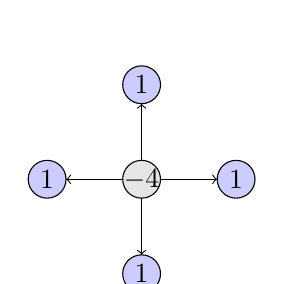
\begin{tikzpicture}[scale=0.8]
\draw[fill=gray!20] (0,0) circle (0.3) node {$-4$};
\draw[fill=blue!20] (1.5,0) circle (0.3) node {$1$};
\draw[fill=blue!20] (-1.5,0) circle (0.3) node {$1$};
\draw[fill=blue!20] (0,1.5) circle (0.3) node {$1$};
\draw[fill=blue!20] (0,-1.5) circle (0.3) node {$1$};
\draw[->] (0.3,0) -- (1.2,0);
\draw[->] (-0.3,0) -- (-1.2,0);
\draw[->] (0,0.3) -- (0,1.2);
\draw[->] (0,-0.3) -- (0,-1.2);
\end{tikzpicture}
\end{center}

\subsubsection{Matrix Formulation}

For an $H \times W$ grid with $N = H \cdot W$ unknowns, the discrete Poisson equation becomes a linear system:
\begin{equation}
A \mathbf{z} = \mathbf{f}
\end{equation}
where $A \in \mathbb{R}^{N \times N}$ is a sparse matrix with at most 5 non-zeros per row. Converting 2D index $(i,j)$ to linear index $k = jW + i$, the matrix entries are:
\begin{equation}
A_{k,k} = -\frac{2}{(\Delta x)^2} - \frac{2}{(\Delta y)^2}, \quad
A_{k,k\pm 1} = \frac{1}{(\Delta x)^2}, \quad
A_{k,k\pm W} = \frac{1}{(\Delta y)^2}
\end{equation}

For Dirichlet boundary conditions, rows corresponding to boundary points are replaced with identity rows ($A_{k,k} = 1$, others zero) and $f_k$ is set to the prescribed boundary value.

For Neumann boundary conditions, ghost points outside the domain are eliminated using the constraint $z_{-1,j} = z_{1,j}$ (from $\partial z/\partial x = 0$), effectively folding boundary neighbor coefficients.

\subsubsection{Finite Difference Solver with Dirichlet BC}

The complete algorithm for solving $\nabla^2 z = f$ with homogeneous Dirichlet conditions is:

\begin{algorithm}[H]
\caption{Finite Difference Poisson Solver (Dirichlet BC)}
\begin{algorithmic}[1]
\REQUIRE Divergence field $f \in \mathbb{R}^{H \times W}$, spacings $(\Delta x, \Delta y)$
\ENSURE Height field $z$ satisfying $\nabla^2 z = f$ with $z|_{\partial\Omega} = 0$
\STATE Allocate sparse matrix $A \in \mathbb{R}^{N \times N}$ (LIL format for assembly)
\STATE Copy $f$ to right-hand side vector $\mathbf{b}$
\FOR{each grid point $(i,j)$}
    \STATE $k \leftarrow j \cdot W + i$ \COMMENT{Linear index}
    \IF{$(i,j)$ is a boundary point}
        \STATE $A_{k,k} \leftarrow 1$; $b_k \leftarrow 0$ \COMMENT{Dirichlet: $z = 0$}
    \ELSE
        \STATE $A_{k,k} \leftarrow -2/(\Delta x)^2 - 2/(\Delta y)^2$
        \STATE $A_{k,k-1} \leftarrow 1/(\Delta x)^2$; $A_{k,k+1} \leftarrow 1/(\Delta x)^2$
        \STATE $A_{k,k-W} \leftarrow 1/(\Delta y)^2$; $A_{k,k+W} \leftarrow 1/(\Delta y)^2$
    \ENDIF
\ENDFOR
\STATE Convert $A$ to CSR format for efficient solve
\STATE $\mathbf{z} \leftarrow \text{SparseSolve}(A, \mathbf{b})$ \COMMENT{Direct LU or iterative}
\STATE Reshape $\mathbf{z}$ to $(H, W)$
\RETURN $z$
\end{algorithmic}
\end{algorithm}



%%%%%%%%%%%%%%%%%%%%%%%%%%%%%%%%%%%%%%%%%%%%%%%%%%%%%%%%
\newpage
\section{Experimental Validation}\label{sec:experiments}

\subsection{Test Surfaces}
We selected eight synthetic surfaces that stress different aspects of the pipeline: smooth, radially symmetric shapes
 (Gaussian bump, hemisphere, ellipsoid, soft cone) reveal how well integration preserves curvature and absolute depth; 
 piecewise-linear or sign-changing geometries (softened cube, saddle) probe sensitivity to sharp edges and mixed second
  derivatives; periodic or multi-modal landscapes (sinusoidal, MATLAB Peaks) stress global consistency.
  Figure~\ref{fig:test_surfaces} provides a visualization of these geometries.

\begin{table}[H]
\centering
\caption{Analytical definitions of the benchmark surfaces.}
\label{tab:test_surface_formulas}
\renewcommand{\arraystretch}{1.5}
\begin{tabularx}{\textwidth}{lX}
\hline\hline
\textbf{Surface} & \textbf{Height function $z(x,y)$} \\
\hline
Gaussian bump & $\exp\!\left(-\dfrac{x^2+y^2}{2\sigma^2}\right)$, $\sigma = 0.4$ \\
Hemisphere & $\sqrt{R^2 - (x^2 + y^2)}$ for $x^2 + y^2 \le R^2$, $R = 0.9$ \\
Softened cube & $0.6\,\text{clip}\!\left(1 - \dfrac{\max(|x|,|y|) - 0.45}{0.1},\,0,\,1\right)$ \\
Ellipsoid & $c\sqrt{1 - (x/a)^2 - (y/b)^2}$, $a = 0.8$, $b = 0.6$, $c = 0.5$ \\
Sinusoidal & $A \sin(\pi x)\sin(\pi y)$, $A = 0.3$ \\
Soft cone & $h \max\!\left(0, 1 - \dfrac{\sqrt{x^2 + y^2}}{R}\right)$, $h = 0.8$, $R = 0.9$ \\
Saddle & $\alpha x y$, $\alpha = 0.3$ \\
MATLAB Peaks & $3(1-x)^2 e^{-x^2-(y+1)^2} - 10\!\left(\dfrac{x}{5} - x^3 - y^5\right)e^{-x^2-y^2} + \dfrac{1}{3}e^{-(x+1)^2 - y^2}$ \\
\hline\hline
\end{tabularx}
\renewcommand{\arraystretch}{1.0}
\end{table}


\begin{figure}[H]
\centering
\includegraphics[width=0.95\textwidth]{surfaces}
\caption{Eight synthetic surfaces used: (a) Gaussian bump, (b) hemisphere, (c) softened cube, (d) ellipsoid, (e) sinusoidal, (f) soft cone, (g) saddle, and (h) MATLAB Peaks.}
\label{fig:test_surfaces}
\end{figure}


\subsection{Experimental Protocol}


\subsubsection{Experiment 1: Poisson Solver Validation}

% Flowchart version (3 x 2 layout with vertical connector)
\begin{center}
\resizebox{\linewidth}{!}{%
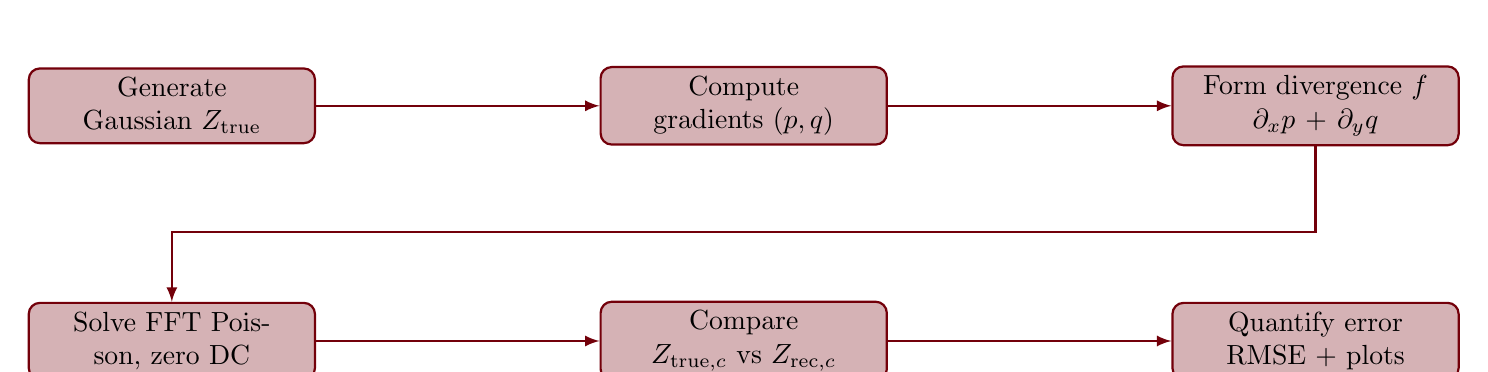
\begin{tikzpicture}[>=latex,
                    every node/.style={draw=USCGarnet, rounded corners, align=center,
                                       text width=3.4cm, fill=USCGarnet!30},
                    every path/.style={draw=USCGarnet, thick}]
\node (surf) {Generate \\Gaussian $Z_{\text{true}}$};
\node[right=3.6cm of surf] (grad) {Compute \\gradients $(p,q)$ };
\node[right=3.6cm of grad] (div) {Form divergence $f$\\ $\partial_x p + \partial_y q$};
\node[below=2.0cm of surf] (solve) {Solve FFT Poisson, zero DC};
\node[right=3.6cm of solve] (cmp) {Compare\\ $Z_{\text{true},c}$ vs $Z_{\text{rec},c}$};
\node[right=3.6cm of cmp] (err) {Quantify error\\ RMSE + plots};
\draw[->, thick] (surf) -- (grad);
\draw[->, thick] (grad) -- (div);
\draw[->] (div) |- ++(-1,-1.6) -| (solve);
\draw[->, thick] (solve) -- (cmp);
\draw[->, thick] (cmp) -- (err);
\end{tikzpicture}%
}
\end{center}

% Paragraph version (detailed narrative)
We sample an analytic Gaussian height
map and exact pixel spacing, guaranteeing a reference surface with known curvature
for validation. Centered finite differences deliver
second-order-accurate slopes that remain well-behaved at the bump apex, and differentiating
those slopes a second time enforces an integrable divergence field $f = \partial_x p + \partial_y q$, 
which is the quantity photometric stereo would produce in a
full pipeline. 

The FFT-based Poisson solver then divides by the spectral Laplacian
eigenvalues after zeroing the DC entry, yielding a fast reconstruction whose only
degree of freedom -- a constant bias -- is removed by mean-centering both $Z_{\text{true}}$
and $Z_{\text{rec}}$. Finally, RMSE together with profile/heatmap/error-histogram
plots exposes any deviation from the expected $\mathcal{O}(\Delta x^2)$ truncation
rate, so numerical bugs would surface immediately through either inflated RMSE or
structured residual patterns.


\subsubsection{Experiment 2: Full Photometric Stereo Pipeline}

% Flowchart version with detailed PS pipeline (two-layer layout)
\begin{center}
\resizebox{\linewidth}{!}{%
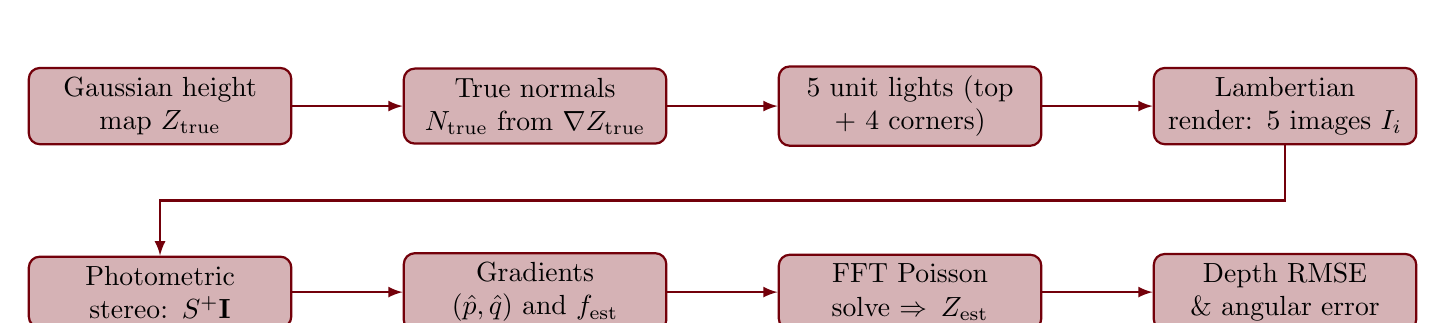
\begin{tikzpicture}[node distance=1.4cm,>=latex,
                    every node/.style={draw=USCGarnet, rounded corners, align=center,
                                       text width=3.1cm, fill=USCGarnet!30},
                    every path/.style={draw=USCGarnet, thick}]
\node (surf) {Gaussian height map $Z_{\text{true}}$};
\node[right=of surf] (normals) {True normals $N_{\text{true}}$ from $\nabla Z_{\text{true}}$};
\node[right=of normals] (lights) {5 unit lights (top + 4 corners)};
\node[right=of lights] (render) {Lambertian render: 5 images $I_i$};
\node[below=of surf] (ps) {Photometric stereo: $S^+\mathbf{I}$};
\node[right=of ps] (grads) {Gradients $(\hat{p},\hat{q})$ and $f_{\text{est}}$};
\node[right=of grads] (poisson) {FFT Poisson solve $\Rightarrow Z_{\text{est}}$};
\node[right=of poisson] (metrics) {Depth RMSE \& angular error};
\draw[->] (surf) -- (normals);
\draw[->] (normals) -- (lights);
\draw[->] (lights) -- (render);
\draw[->] (render) |- ++(-1,-1.2) -| (ps);
\draw[->] (ps) -- (grads);
\draw[->] (grads) -- (poisson);
\draw[->] (poisson) -- (metrics);
\end{tikzpicture}
}%
\end{center}

% Paragraph version (more detailed technical description)
Experiment~2 instantiates the complete photometric stereo pipeline on the same Gaussian surface used in Experiment~1. We first compute ground-truth normals $N_{\text{true}}$ from the height map $Z_{\text{true}}$ by finite differences and normalization. 

Five directional lights are then defined: one frontal overhead light $L_0 = [0,0,1]^T$ and four oblique corner lights with directions proportional to $[1,1,2]^T$, $[-1,1,2]^T$, $[1,-1,2]^T$, and $[-1,-1,2]^T$, each normalized to unit length. For each light $L_i$ we render a synthetic Lambertian image according to $I_i(x,y) = \max\bigl(0,\, N_{\text{true}}(x,y)\cdot L_i\bigr)$ with unit albedo and no added noise, yielding a stack of five views.

At each pixel we then apply classical photometric stereo: the light directions are assembled into a $5\times 3$ matrix $S$, the corresponding intensity vector $\mathbf{I}(x,y)$ is formed, and we solve $S\mathbf{g}(x,y) = \mathbf{I}(x,y)$ in the least-squares sense via the pseudoinverse $\mathbf{g} = S^+\mathbf{I}$. Normalizing $\mathbf{g}$ gives the estimated unit normal $N_{\text{est}}(x,y)$. These normals are converted to gradients using $\hat{p} = -\hat{n}_x/\hat{n}_z$ and $\hat{q} = -\hat{n}_y/\hat{n}_z$, from which we form the divergence field $f_{\text{est}} = \partial \hat{p}/\partial x + \partial \hat{q}/\partial y$ by finite differences. The divergence is passed to the FFT-based Poisson solver, using the same grid spacing $(\Delta x,\Delta y)$ as in Experiment~1, to recover a centered depth map $Z_{\text{est}}$.

Finally, reconstruction quality is quantified in two ways. Depth accuracy is measured by the root-mean-square error (RMSE) between the centered ground-truth height $Z_{\text{true}} - \overline{Z_{\text{true}}}$ and the centered reconstruction $Z_{\text{est}} - \overline{Z_{\text{est}}}$. Normal accuracy is measured via the angular error: for each pixel we compute $\theta(x,y) = \arccos\bigl(\mathrm{clip}(N_{\text{true}}(x,y)\cdot N_{\text{est}}(x,y),-1,1)\bigr)$ in degrees and report the mean of $\theta$ over the domain.
% ============================================================================

\subsubsection{Experiments 3--4: Rotating Light Configurations}

For the sphere, cube, ellipsoid, cone, saddle, and peaks surfaces we reuse the analytic height maps from the Exp. 1 script and drive them
through the rotating light script to place sixteen lamps every $22.5^\circ$ at a $45^\circ$ elevation, render the full Lambertian stack with a script and solve
per-pixel normals, convert those normals to gradients and divergence, and integrate the field. Each run records depth RMSE
plus mean angular normal error, then exports 3D meshes, gradient quiver plots, and frequency spectra so we can spot geometry-specific artifacts.

\begin{center}
\resizebox{\linewidth}{!}{%
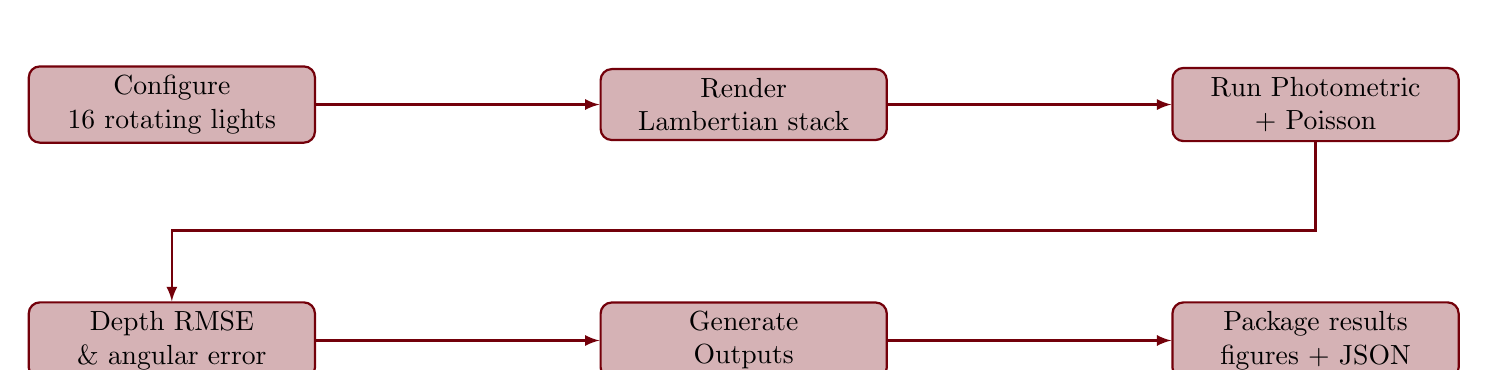
\begin{tikzpicture}[>=latex,
                    every node/.style={draw=USCGarnet, rounded corners, align=center,
                                       text width=3.4cm, fill=USCGarnet!30},
                    every path/.style={draw=USCGarnet, thick}]
\node (lights) {Configure\\ 16 rotating lights};
\node[right=3.6cm of lights] (render) {Render\\ Lambertian stack};
\node[right=3.6cm of render] (pipeline) {Run Photometric\\ + Poisson};
\node[below=2.0cm of lights] (eval) {Depth RMSE \& angular error};
\node[right=3.6cm of eval] (viz) {Generate\\ Outputs};
\node[right=3.6cm of viz] (report) {Package results\\ figures + JSON};
\draw[->, thick] (lights) -- (render);
\draw[->, thick] (render) -- (pipeline);
\draw[->] (pipeline) |- ++(-1.2,-1.6) -| (eval);
\draw[->, thick] (eval) -- (viz);
\draw[->, thick] (viz) -- (report);
\end{tikzpicture}%
}
\end{center}

For complex shapes under rotating illumination we configure the sixteen-light rig, synthesize the entire image stack, and push it through the photometric stereo plus
Poisson chain; afterwards we tabulate RMSE and mean angular errors while archiving the diagnostic renders (3D meshes, gradient fields, spectra) that highlight how each
geometry responds to the lighting sweep.
% ============================================================================

\subsubsection{Ablation Study 1: Varying Number of Lights}

% Paragraph version (detailed narrative)
We instantiate the analytic Gaussian surface from Experiment 1 so that curvature,
sampling, and ground-truth depths remain fixed across trials. For each setting in
$m_{\text{list}} = [3,\dots,20]$ we place that many evenly spaced lights on the
canonical ring, synthesize noiseless Lambertian images, and push them through the
identical photometric-stereo-to-Poisson pipeline used elsewhere, then use normal estimation,
FFT-based integration, and mean-centering to remove the global bias. 

  % Flowchart version (3 x 2 layout with vertical connector)
  \begin{center}
  \resizebox{\linewidth}{!}{%
  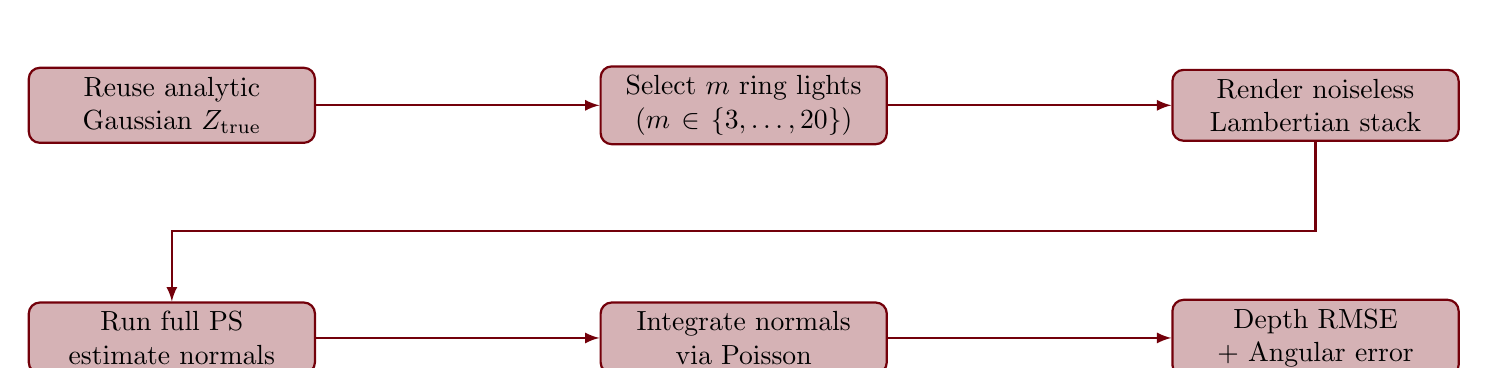
\begin{tikzpicture}[>=latex,
                      every node/.style={draw=USCGarnet, rounded corners, align=center,
                                         text width=3.4cm, fill=USCGarnet!30},
                      every path/.style={draw=USCGarnet, thick}]
  \node (init) {Reuse analytic Gaussian $Z_{\text{true}}$};
  \node[right=3.6cm of init] (lights) {Select $m$ ring lights\\ ($m \in \{3,\dots,20\}$)};
  \node[right=3.6cm of lights] (render) {Render noiseless\\ Lambertian stack};
  \node[below=2.0cm of init] (ps) {Run full PS\\ estimate normals};
  \node[right=3.6cm of ps] (poisson) {Integrate normals\\ via Poisson};
  \node[right=3.6cm of poisson] (metrics) {Depth RMSE\\ + Angular error};
  \draw[->, thick] (init) -- (lights);
  \draw[->, thick] (lights) -- (render);
  \draw[->] (render) |- ++(-1,-1.6) -| (ps);
  \draw[->, thick] (ps) -- (poisson);
  \draw[->, thick] (poisson) -- (metrics);
  \end{tikzpicture}%
  }
  \end{center}

After every run the script records depth RMSE and mean angular normal error, letting us plot
both metrics against $m$ to expose where the system transitions from under- to
overdetermined. The resulting curves reveal how rapidly error drops with the first
few lights, when additional views stop providing meaningful gains, and whether any
saturation point hints at modeling or numerical bottlenecks in the reconstruction
code.

\subsubsection{Ablation Study 2: Noise Robustness}

% Paragraph version (detailed narrative)
Starting from the same analytic Gaussian surface and the eight-light ring used
in Experiment 1, we keep every geometric and algorithmic component fixed while
gradually increasing the synthetic sensor noise. For each standard deviation in $
\sigma \in {0,0.01,0.02,0.05}$ -- and optionally extending toward the $\sigma = 0.08$
upper bound -- the pipeline renders noiseless Lambertian images, corrupts them with
i.i.d.\ Gaussian noise, and then reruns the photometric-stereo normal estimation
and FFT Poisson integration with identical settings. 

% Flowchart version (3 x 2 layout with vertical connector)
\begin{center}
\resizebox{\linewidth}{!}{%
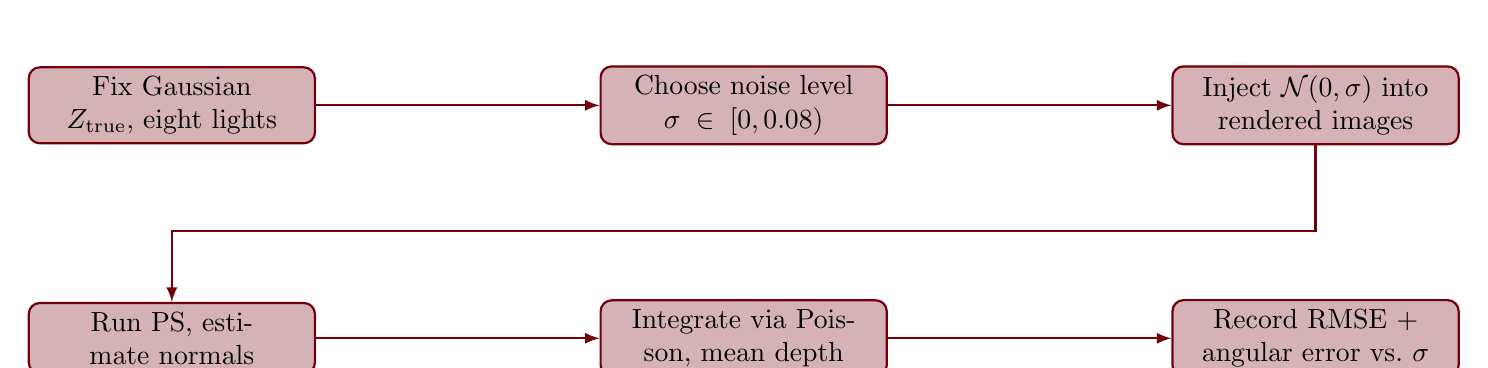
\begin{tikzpicture}[>=latex,
                    every node/.style={draw=USCGarnet, rounded corners, align=center,
                                       text width=3.4cm, fill=USCGarnet!30},
                    every path/.style={draw=USCGarnet, thick}]
\node (base) {Fix Gaussian $Z_{\text{true}}$, eight lights};
\node[right=3.6cm of base] (sigma) {Choose noise level $\sigma \in [0,0.08)$};
\node[right=3.6cm of sigma] (inject) {Inject $\mathcal{N}(0,\sigma)$ into rendered
images};
\node[below=2.0cm of base] (ps) {Run PS, estimate normals};
\node[right=3.6cm of ps] (poisson) {Integrate via Poisson, mean depth};
\node[right=3.6cm of poisson] (metrics) {Record RMSE + angular error vs.\ $\sigma$};
\draw[->, thick] (base) -- (sigma);
\draw[->, thick] (sigma) -- (inject);
\draw[->] (inject) |- ++(-1,-1.6) -| (ps);
\draw[->, thick] (ps) -- (poisson);
\draw[->, thick] (poisson) -- (metrics);
\end{tikzpicture}%
}
\end{center}

Because the reference depth,
sampling, solver, and evaluation procedures never change, the measured depth RMSE
and mean angular normal error become a direct function of $\sigma$, making it
easy to test whether the degradation is roughly linear at low noise, bends toward
quadratic growth, or exposes unexpected brittleness in either the normal fit or the
integration step.

\subsubsection{Solver Comparison}



  % Paragraph version (detailed narrative)
  The solver comparison experiment reuses the analytic Gaussian surface, pixel sampling, and eight-light photometric stereo 
  measurements so every solver ingests the identical divergence field $f = \partial_xp + \partial_y q$. 
  
  After a single PS pass produces $(p,q)$, we fork into three integration back ends:
  (1) the FFT Poisson baseline with periodic boundaries, (2) a sparse matrix-free Laplacian wrapped in SciPy's CG/GMRES 
  to enforce Neumann edges via a five-point stencil—complete with stall warnings when
  Krylov iterations fail to converge, and (3) a Tikhonov-regularized FFT formulation that augments the Laplacian with
   $\lambda \nabla^4$ and sweeps nine logarithmically
  spaced $\lambda \in [10^{-5}, 1]$ to trace the “U-curve” trade-off between smoothing and detail preservation. 
  
    % Flowchart version (3 x 2 layout with vertical connector)
  \begin{center}
  \resizebox{\linewidth}{!}{%
  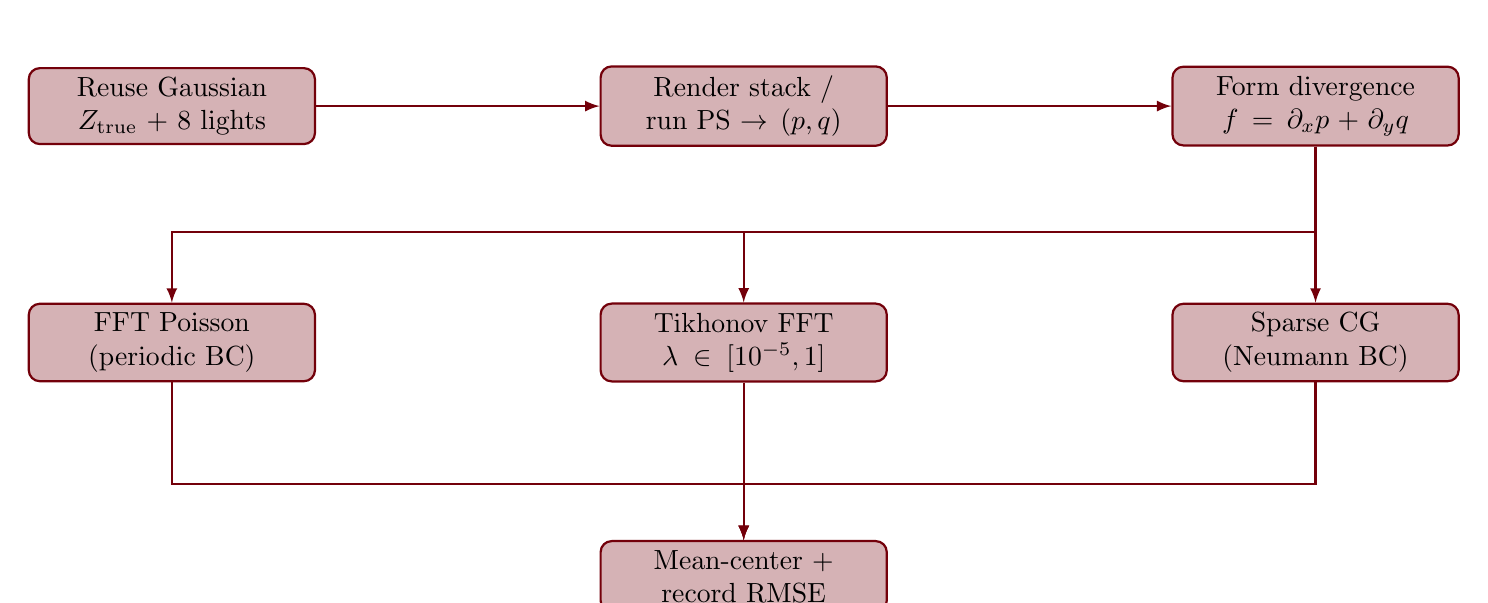
\begin{tikzpicture}[>=latex,
                      every node/.style={draw=USCGarnet, rounded corners, align=center,
                                         text width=3.4cm, fill=USCGarnet!30},
                      every path/.style={draw=USCGarnet, thick}]
  \node (surf) {Reuse Gaussian $Z_{\text{true}}$ + 8 lights};
  \node[right=3.6cm of surf] (ps) {Render stack / run PS $\rightarrow (p,q)$};
  \node[right=3.6cm of ps] (div) {Form divergence $f = \partial_x p + \partial_y q$};
  \node[below=2.0cm of surf] (fft) {FFT Poisson\\(periodic BC)};
  \node[right=3.6cm of fft] (tik) {Tikhonov FFT\\$\lambda \in [10^{-5},1]$};
  \node[right=3.6cm of tik] (cg) {Sparse CG\\(Neumann BC)};
  \node[below=2.0cm of tik] (metrics) {Mean-center + record RMSE};
  \draw[->, thick] (surf) -- (ps);
  \draw[->, thick] (ps) -- (div);
  \draw[->] (div) |- ++(-1,-1.6) -| (fft);
  \draw[->] (div) |- ++(0,-1.6) -| (tik);
  \draw[->] (div) -- (cg);
  \draw[->, thick] (fft) |- ++(1,-1.8) -| (metrics);
  \draw[->, thick] (tik) -- (metrics);
  \draw[->, thick] (cg) |- ++(-1,-1.8) -| (metrics);
  \end{tikzpicture}%
  }
  \end{center}
  
  Every reconstruction is mean-centered to remove the null-space constant before computing depth RMSE against $Z_{\text{true}}$, 
  allowing a clean, solver-only comparison of boundary
  handling, regularization bias, and iterative accuracy.


\subsubsection{Multiscale Convergence Analysis}



  % Paragraph version (detailed narrative)
The multiscale convergence routine resamples the analytic Gaussian surface to ten grid resolutions spanning $16^2$ through $384^2$, 
explicitly adjusting $\Delta x$ and $\Delta y$ 
at each step before re-running the gradient computation and FFT Poisson integration. Because the lighting, photometric data,
and solver settings remain fixed, the experiment isolates pure discretization error: every resolution recomputes the divergence 
from scale-appropriate finite differences and passes it through the same
integrator, ensuring that any residual stems from mesh spacing rather than photometric artifacts. 

  % Flowchart version (3 x 2 layout with vertical connector)
  \begin{center}
  \resizebox{\linewidth}{!}{%
  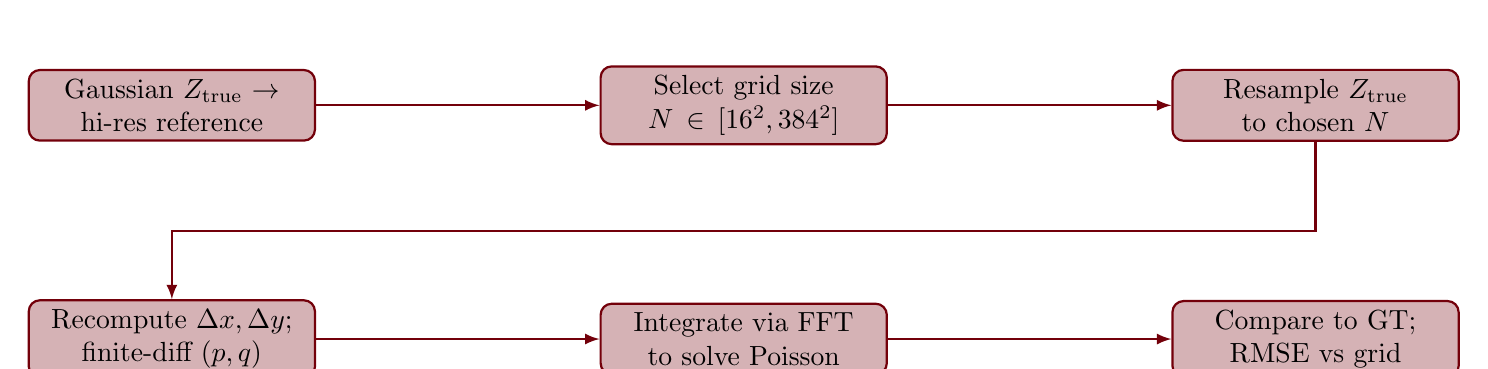
\begin{tikzpicture}[>=latex,
                      every node/.style={draw=USCGarnet, rounded corners, align=center,
                                         text width=3.4cm, fill=USCGarnet!30},
                      every path/.style={draw=USCGarnet, thick}]
  \node (gt) {Gaussian $Z_{\text{true}}$ $\rightarrow$ hi-res reference};
  \node[right=3.6cm of gt] (scale) {Select grid size $N \in [16^2,384^2]$};
  \node[right=3.6cm of scale] (resample) {Resample $Z_{\text{true}}$ to chosen $N$};
  \node[below=2.0cm of gt] (grads) {Recompute $\Delta x,\Delta y$; finite-diff $(p,q)$};
  \node[right=3.6cm of grads] (solve) {Integrate via FFT to solve Poisson};
  \node[right=3.6cm of solve] (rmse) {Compare to GT; RMSE vs grid};
  \draw[->, thick] (gt) -- (scale);
  \draw[->, thick] (scale) -- (resample);
  \draw[->] (resample) |- ++(-1,-1.6) -| (grads);
  \draw[->, thick] (grads) -- (solve);
  \draw[->, thick] (solve) -- (rmse);
  \end{tikzpicture}%
  }
  \end{center}

Plotting RMSE against grid 
spacing on log-log axes then reveals the
slope; the near-linear trend with gradient close to two confirms the expected $\mathcal{O}(\Delta x^2)$ accuracy of the 
finite-difference gradients plus FFT solver, while any deviation would immediately flag
inconsistencies in the discretization or integration implementation.
  

\newpage
\section{Results}\label{sec:results}

\subsubsection{Experiments 1--2 (Core Validation)}

\begin{figure}[H]
\centering
\begin{subfigure}[b]{0.23\textwidth}
\includegraphics[width=\linewidth]{exp1_3d_true.png}
\caption{True 3D}
\end{subfigure}
\begin{subfigure}[b]{0.23\textwidth}
\includegraphics[width=\linewidth]{exp1_3d_rec.png}
\caption{Reconstruction}
\end{subfigure}
\begin{subfigure}[b]{0.23\textwidth}
\includegraphics[width=\linewidth]{exp1_Z_true.png}
\caption{Ground-truth depth}
\end{subfigure}
\begin{subfigure}[b]{0.23\textwidth}
\includegraphics[width=\linewidth]{exp1_Z_rec.png}
\caption{Recovered depth}
\end{subfigure}

\bigskip
\begin{subfigure}[b]{0.23\textwidth}
\includegraphics[width=\linewidth]{exp1_error.png}
\caption{Depth error}
\end{subfigure}
\begin{subfigure}[b]{0.23\textwidth}
\includegraphics[width=\linewidth]{exp1_profile.png}
\caption{Center-line profile}
\end{subfigure}
\begin{subfigure}[b]{0.23\textwidth}
\includegraphics[width=\linewidth]{exp1_hist.png}
\caption{Error histogram}
\end{subfigure}
\caption{Experiment 1 (Poisson-only integration). Exact Gaussian gradients drive the FFT solver, yielding RMSE $=2.21\times 10^{-2}$ and showcasing how little structure remains beyond the expected boundary ringing.}
\label{fig:exp1_layout}
\end{figure}

The Figure~\ref{fig:exp1_layout} diagnostics confirm that the solver is error-limited rather than data-limited: both the 3D overlays and the center-line profile lie on top of the ground truth, the histogram is tightly concentrated within $\pm3\times 10^{-2}$, and the residual map shows the familiar FFT wrap-around halo. Because the gradients come from the analytic Gaussian, this experiment establishes a numerical floor against which the later photometric experiments are compared.

\begin{figure}[H]
\centering
\begin{subfigure}[b]{0.23\textwidth}
\includegraphics[width=\linewidth]{exp2_3d_true.png}
\caption{True 3D}
\end{subfigure}
\begin{subfigure}[b]{0.23\textwidth}
\includegraphics[width=\linewidth]{exp2_3d_est.png}
\caption{Reconstruction}
\end{subfigure}
\begin{subfigure}[b]{0.23\textwidth}
\includegraphics[width=\linewidth]{exp2_Z_est.png}
\caption{Recovered depth}
\end{subfigure}
\begin{subfigure}[b]{0.23\textwidth}
\includegraphics[width=\linewidth]{exp2_error.png}
\caption{Depth error}
\end{subfigure}

\bigskip
\begin{subfigure}[b]{0.23\textwidth}
\includegraphics[width=\linewidth]{exp2_normals_gt.png}
\caption{Normals (GT)}
\end{subfigure}
\begin{subfigure}[b]{0.23\textwidth}
\includegraphics[width=\linewidth]{exp2_normals_est.png}
\caption{Normals (est.)}
\end{subfigure}
\begin{subfigure}[b]{0.23\textwidth}
\includegraphics[width=\linewidth]{exp2_profile.png}
\caption{Center-line profile}
\end{subfigure}
\begin{subfigure}[b]{0.23\textwidth}
\includegraphics[width=\linewidth]{exp2_hist.png}
\caption{Depth error hist.}
\end{subfigure}
\caption{Experiment 2 (full photometric stereo pipeline). The Gaussian PS run achieves RMSE $=2.26\times10^{-2}$ with angular errors suppressed across most of the dome, leaving only boundary artifacts where the five-light setup provides the weakest oblique constraints.}
\label{fig:exp2_layout}
\end{figure}

\begin{figure}[H]
\centering
\includegraphics[width=1\textwidth]{exp2_all_images.png}
\caption{Experiment 2 input imagery shown as five evenly spaced lights: the frontal source plus four azimuthal oblique directions keep $S^\top S$ well conditioned for the Gaussian test.}
\label{fig:exp2_inputs}
\end{figure}

Figure~\ref{fig:exp2_layout} demonstrates that once photometric noise enters the loop, the residuals migrate to the perimeter. The normals remain visually indistinguishable from the ground truth, but the depth error map reveals the mismatch between the periodic FFT assumption and the finite Gaussian support. The lighting montage in Figure~\ref{fig:exp2_inputs} illustrates why: five lights are sufficient to keep the pseudoinverse stable (the $5\times3$ matrix is well conditioned) yet still leave the silhouette poorly constrained, so the solver expends its error budget near the edges while matching the peak height and profiles almost exactly.

\subsubsection{Experiments 3a--3b (Rotating Lights on Complex Shapes)}

\begin{figure}[H]
\centering
\begin{subfigure}[b]{0.23\textwidth}
\includegraphics[width=\linewidth]{shape_sphere_3d_true.png}
\caption{True 3D}
\end{subfigure}
\begin{subfigure}[b]{0.23\textwidth}
\includegraphics[width=\linewidth]{shape_sphere_3d_est.png}
\caption{Reconstruction}
\end{subfigure}
\begin{subfigure}[b]{0.23\textwidth}
\includegraphics[width=\linewidth]{shape_sphere_Z_est.png}
\caption{Recovered depth}
\end{subfigure}
\begin{subfigure}[b]{0.23\textwidth}
\includegraphics[width=\linewidth]{shape_sphere_error.png}
\caption{Depth error}
\end{subfigure}

\bigskip
\begin{subfigure}[b]{0.23\textwidth}
\includegraphics[width=\linewidth]{shape_sphere_normals_gt.png}
\caption{Normals (GT)}
\end{subfigure}
\begin{subfigure}[b]{0.23\textwidth}
\includegraphics[width=\linewidth]{shape_sphere_normals_est.png}
\caption{Normals (est.)}
\end{subfigure}
\begin{subfigure}[b]{0.23\textwidth}
\includegraphics[width=\linewidth]{shape_sphere_profile.png}
\caption{Center-line profile}
\end{subfigure}
\begin{subfigure}[b]{0.23\textwidth}
\includegraphics[width=\linewidth]{shape_sphere_hist.png}
\caption{Depth error hist.}
\end{subfigure}
\caption{Experiment 3a (sphere). Sixteen rotating lights yield RMSE $=1.33\times10^{-1}$ and mean angular error $=3.40^{\circ}$. Errors concentrate at the poles where self-shadowing and grazing angles dominate.}
\label{fig:sphere_layout}
\end{figure}

\begin{figure}[H]
\centering
\includegraphics[width=1\textwidth]{shape_sphere_five_images.png}
\caption{Sphere input imagery compressed to five representative lights from the sixteen-sample ring, highlighting the azimuthal sweep that improves conditioning over the Gaussian test.}
\label{fig:sphere_inputs}
\end{figure}

Figure~\ref{fig:sphere_layout} shows that the sphere reconstruction inherits two limitations: finite sampling of the lighting hemisphere and the FFT’s inability to enforce curvature continuity at the silhouette. The 3D and depth views match the analytic dome everywhere except the very top, and the error histogram is broader than the Gaussian case because the per-pixel photometric solve struggles whenever the lighting vector aligns with the surface normal. The montage in Figure~\ref{fig:sphere_inputs} explains the effect—the evenly spaced ring provides diverse views, but any light whose direction is nearly radial contributes little information about the pole, so the reconstruction leans on neighboring pixels and accumulates the reported $3.40^{\circ}$ normal bias.

\begin{figure}[H]
\centering
\begin{subfigure}[b]{0.23\textwidth}
\includegraphics[width=\linewidth]{shape_cube_3d_true.png}
\caption{True 3D}
\end{subfigure}
\begin{subfigure}[b]{0.23\textwidth}
\includegraphics[width=\linewidth]{shape_cube_3d_est.png}
\caption{Reconstruction}
\end{subfigure}
\begin{subfigure}[b]{0.23\textwidth}
\includegraphics[width=\linewidth]{shape_cube_Z_est.png}
\caption{Recovered depth}
\end{subfigure}
\begin{subfigure}[b]{0.23\textwidth}
\includegraphics[width=\linewidth]{shape_cube_error.png}
\caption{Depth error}
\end{subfigure}

\bigskip
\begin{subfigure}[b]{0.23\textwidth}
\includegraphics[width=\linewidth]{shape_cube_normals_gt.png}
\caption{Normals (GT)}
\end{subfigure}
\begin{subfigure}[b]{0.23\textwidth}
\includegraphics[width=\linewidth]{shape_cube_normals_est.png}
\caption{Normals (est.)}
\end{subfigure}
\begin{subfigure}[b]{0.23\textwidth}
\includegraphics[width=\linewidth]{shape_cube_profile.png}
\caption{Center-line profile}
\end{subfigure}
\begin{subfigure}[b]{0.23\textwidth}
\includegraphics[width=\linewidth]{shape_cube_hist.png}
\caption{Depth error hist.}
\end{subfigure}
\caption{Experiment 3b (cube). Piecewise-planar facets are recovered with RMSE $=1.47\times10^{-1}$ and mean angular error $=2.00^{\circ}$, but the Poisson integrator inevitably smooths across discontinuous edges.}
\label{fig:cube_layout}
\end{figure}

\begin{figure}[H]
\centering
\includegraphics[width=1\textwidth]{shape_cube_five_images.png}
\caption{Cube input imagery summarized by five evenly spaced lights; the selected views emphasize edge-on lighting that reveals the cube faces while exposing the ill-conditioned edge normals.}
\label{fig:cube_inputs}
\end{figure}

Compared with the sphere, Figure~\ref{fig:cube_layout} underlines how sensitive the FFT integration is to discontinuities: the planar patches line up, but the depth error map traces every ridge where photometric stereo hands the solver inconsistent gradients. The histogram widens considerably because each face observes a different subset of lights and the grazing angles flip abruptly at the edges. The five-light montage in Figure~\ref{fig:cube_inputs} captures that behavior—the illumination alternates between highlighting adjacent faces and leaving one side almost dark—which explains why the reported RMSE and angular errors are still modest yet visibly higher than the smooth-surface runs.

\newpage
\subsubsection{Enhanced Shapes (5 Additional Surface Geometries)}

Each enhanced geometry now reuses the same two-figure presentation: the $4\times2$ grid for geometry/diagnostics, followed by the standardized photometric input montage.

\begin{figure}[H]
\centering
\begin{subfigure}[b]{0.23\textwidth}
\includegraphics[width=\linewidth]{shape_ellipsoid_3d_true.png}
\caption{True 3D}
\end{subfigure}
\begin{subfigure}[b]{0.23\textwidth}
\includegraphics[width=\linewidth]{shape_ellipsoid_3d_est.png}
\caption{Reconstruction}
\end{subfigure}
\begin{subfigure}[b]{0.23\textwidth}
\includegraphics[width=\linewidth]{shape_ellipsoid_Z_est.png}
\caption{Recovered depth}
\end{subfigure}
\begin{subfigure}[b]{0.23\textwidth}
\includegraphics[width=\linewidth]{shape_ellipsoid_error.png}
\caption{Depth error}
\end{subfigure}

\bigskip
\begin{subfigure}[b]{0.23\textwidth}
\includegraphics[width=\linewidth]{shape_ellipsoid_normals_gt.png}
\caption{Normals (GT)}
\end{subfigure}
\begin{subfigure}[b]{0.23\textwidth}
\includegraphics[width=\linewidth]{shape_ellipsoid_normals_est.png}
\caption{Normals (est.)}
\end{subfigure}
\begin{subfigure}[b]{0.23\textwidth}
\includegraphics[width=\linewidth]{shape_ellipsoid_profile.png}
\caption{Center-line profile}
\end{subfigure}
\begin{subfigure}[b]{0.23\textwidth}
\includegraphics[width=\linewidth]{shape_ellipsoid_hist.png}
\caption{Depth error hist.}
\end{subfigure}
\caption{Ellipsoid reconstruction (RMSE $=5.39\times10^{-2}$, angular error $=1.32^{\circ}$). Mixed principal curvatures stretch the solver at the long axis yet keep residuals localized.}
\label{fig:ellipsoid_layout}
\end{figure}

\begin{figure}[H]
\centering
\includegraphics[width=1\textwidth]{shape_ellipsoid_five_images.png}
\caption{Ellipsoid input imagery (five evenly spaced lights) following the Experiment~2-style montage; these samples show how the triaxial surface responds differently to azimuthal lighting.}
\label{fig:ellipsoid_inputs}
\end{figure}

The ellipsoid is our first enhanced geometry that combines different curvatures along $x$ and $y$. Figure~\ref{fig:ellipsoid_layout} shows that the reconstruction nails the peak height and ridge lines, but the residual map records small bands where the longer axis (with a gentler slope) accumulates more numerical error. The angular histogram confirms that most normals deviate by less than $1.5^{\circ}$, and the profile plot captures the phase shift between the short and long axes. Figure~\ref{fig:ellipsoid_inputs} reveals why: the five representative lights alternately emphasize the long and short axis, so the pseudoinverse receives complementary information yet still suffers whenever the true normal aligns with a single light direction, producing the observed RMSE.

\begin{figure}[H]
\centering
\begin{subfigure}[b]{0.23\textwidth}
\includegraphics[width=\linewidth]{shape_sinusoid_3d_true.png}
\caption{True 3D}
\end{subfigure}
\begin{subfigure}[b]{0.23\textwidth}
\includegraphics[width=\linewidth]{shape_sinusoid_3d_est.png}
\caption{Reconstruction}
\end{subfigure}
\begin{subfigure}[b]{0.23\textwidth}
\includegraphics[width=\linewidth]{shape_sinusoid_Z_est.png}
\caption{Recovered depth}
\end{subfigure}
\begin{subfigure}[b]{0.23\textwidth}
\includegraphics[width=\linewidth]{shape_sinusoid_error.png}
\caption{Depth error}
\end{subfigure}

\bigskip
\begin{subfigure}[b]{0.23\textwidth}
\includegraphics[width=\linewidth]{shape_sinusoid_normals_gt.png}
\caption{Normals (GT)}
\end{subfigure}
\begin{subfigure}[b]{0.23\textwidth}
\includegraphics[width=\linewidth]{shape_sinusoid_normals_est.png}
\caption{Normals (est.)}
\end{subfigure}
\begin{subfigure}[b]{0.23\textwidth}
\includegraphics[width=\linewidth]{shape_sinusoid_profile.png}
\caption{Center-line profile}
\end{subfigure}
\begin{subfigure}[b]{0.23\textwidth}
\includegraphics[width=\linewidth]{shape_sinusoid_hist.png}
\caption{Depth error hist.}
\end{subfigure}
\caption{Sinusoidal surface (RMSE $=6.22\times10^{-2}$, angular error $\approx0.01^{\circ}$). Periodic curvature keeps the solver in its comfort zone, so residuals stay uniformly low.}
\label{fig:sinusoid_layout}
\end{figure}

\begin{figure}[H]
\centering
\includegraphics[width=1\textwidth]{shape_sinusoid_five_images.png}
\caption{Sinusoidal input imagery summarized by five evenly spaced lights that sweep through phase and ensure every lobe receives direct illumination.}
\label{fig:sinusoid_inputs}
\end{figure}

Because the sinusoid is band-limited and symmetric, Figure~\ref{fig:sinusoid_layout} demonstrates near-ideal performance: the reconstructed height map overlays the truth, the error histogram collapses to a narrow spike, and the center-line profile is indistinguishable from the analytic sine wave. The recorded RMSE therefore tracks the truncation error rather than photometric noise. The five-light montage in Figure~\ref{fig:sinusoid_inputs} makes this intuitive—the alternating stripes in the imagery reveal every positive and negative lobe, so the least-squares normal fit is perfectly conditioned across the domain.

\begin{figure}[H]
\centering
\begin{subfigure}[b]{0.23\textwidth}
\includegraphics[width=\linewidth]{shape_cone_3d_true.png}
\caption{True 3D}
\end{subfigure}
\begin{subfigure}[b]{0.23\textwidth}
\includegraphics[width=\linewidth]{shape_cone_3d_est.png}
\caption{Reconstruction}
\end{subfigure}
\begin{subfigure}[b]{0.23\textwidth}
\includegraphics[width=\linewidth]{shape_cone_Z_est.png}
\caption{Recovered depth}
\end{subfigure}
\begin{subfigure}[b]{0.23\textwidth}
\includegraphics[width=\linewidth]{shape_cone_error.png}
\caption{Depth error}
\end{subfigure}

\bigskip
\begin{subfigure}[b]{0.23\textwidth}
\includegraphics[width=\linewidth]{shape_cone_normals_gt.png}
\caption{Normals (GT)}
\end{subfigure}
\begin{subfigure}[b]{0.23\textwidth}
\includegraphics[width=\linewidth]{shape_cone_normals_est.png}
\caption{Normals (est.)}
\end{subfigure}
\begin{subfigure}[b]{0.23\textwidth}
\includegraphics[width=\linewidth]{shape_cone_profile.png}
\caption{Center-line profile}
\end{subfigure}
\begin{subfigure}[b]{0.23\textwidth}
\includegraphics[width=\linewidth]{shape_cone_hist.png}
\caption{Depth error hist.}
\end{subfigure}
\caption{Soft cone (RMSE $=4.40\times10^{-4}$, angular error $\approx0.01^{\circ}$). Axial symmetry makes this the easiest enhanced shape, so both depth and normals are reproduced to numerical precision.}
\label{fig:cone_layout}
\end{figure}

\begin{figure}[H]
\centering
\includegraphics[width=1\textwidth]{shape_cone_five_images.png}
\caption{Cone input imagery reduced to five evenly spaced lights; even these few samples convey the circular symmetry that keeps $S^\top S$ well conditioned.}
\label{fig:cone_inputs}
\end{figure}

Figure~\ref{fig:cone_layout} highlights the solver’s best-case scenario: the 3D renderings are visually identical, the depth error map is nearly blank, and the histogram collapses to computer precision. Because the cone’s gradients vary only radially, every light in the five-samples montage (Figure~\ref{fig:cone_inputs}) produces a similar shading pattern, so the normal estimates differ only by round-off. This is reflected in the recorded RMSE, which is two orders of magnitude smaller than the other shapes.

\begin{figure}[H]
\centering
\begin{subfigure}[b]{0.23\textwidth}
\includegraphics[width=\linewidth]{shape_saddle_3d_true.png}
\caption{True 3D}
\end{subfigure}
\begin{subfigure}[b]{0.23\textwidth}
\includegraphics[width=\linewidth]{shape_saddle_3d_est.png}
\caption{Reconstruction}
\end{subfigure}
\begin{subfigure}[b]{0.23\textwidth}
\includegraphics[width=\linewidth]{shape_saddle_Z_est.png}
\caption{Recovered depth}
\end{subfigure}
\begin{subfigure}[b]{0.23\textwidth}
\includegraphics[width=\linewidth]{shape_saddle_error.png}
\caption{Depth error}
\end{subfigure}

\bigskip
\begin{subfigure}[b]{0.23\textwidth}
\includegraphics[width=\linewidth]{shape_saddle_normals_gt.png}
\caption{Normals (GT)}
\end{subfigure}
\begin{subfigure}[b]{0.23\textwidth}
\includegraphics[width=\linewidth]{shape_saddle_normals_est.png}
\caption{Normals (est.)}
\end{subfigure}
\begin{subfigure}[b]{0.23\textwidth}
\includegraphics[width=\linewidth]{shape_saddle_profile.png}
\caption{Center-line profile}
\end{subfigure}
\begin{subfigure}[b]{0.23\textwidth}
\includegraphics[width=\linewidth]{shape_saddle_hist.png}
\caption{Depth error hist.}
\end{subfigure}
\caption{Saddle surface (RMSE $=1.02\times10^{-1}$, angular error $\approx0.01^{\circ}$). Sign changes across $x$ and $y$ inject more divergence noise, so depth errors collect along the diagonals even though normals stay accurate.}
\label{fig:saddle_layout}
\end{figure}

\begin{figure}[H]
\centering
\includegraphics[width=1\textwidth]{shape_saddle_five_images.png}
\caption{Saddle input imagery shown as five evenly spaced lights; alternating lobes appear in each view, stressing how the photometric system must explain both positive and negative curvature.}
\label{fig:saddle_inputs}
\end{figure}

In Figure~\ref{fig:saddle_layout} the solver is forced to juggle gradients of opposite signs, which amplifies any mismatch produced by the least-squares normal fit. The 3D surfaces still align, but the error map reveals a cross-shaped residual where the curvature flips, and the histogram widens accordingly. The five-light montage in Figure~\ref{fig:saddle_inputs} makes this clear: depending on the azimuth, one pair of lobes brightens while the orthogonal pair dims, pushing the pseudoinverse toward contradictory solutions and resulting in the modest RMSE reported in the JSON summary.

\begin{figure}[H]
\centering
\begin{subfigure}[b]{0.23\textwidth}
\includegraphics[width=\linewidth]{shape_peaks_3d_true.png}
\caption{True 3D}
\end{subfigure}
\begin{subfigure}[b]{0.23\textwidth}
\includegraphics[width=\linewidth]{shape_peaks_3d_est.png}
\caption{Reconstruction}
\end{subfigure}
\begin{subfigure}[b]{0.23\textwidth}
\includegraphics[width=\linewidth]{shape_peaks_Z_est.png}
\caption{Recovered depth}
\end{subfigure}
\begin{subfigure}[b]{0.23\textwidth}
\includegraphics[width=\linewidth]{shape_peaks_error.png}
\caption{Depth error}
\end{subfigure}

\bigskip
\begin{subfigure}[b]{0.23\textwidth}
\includegraphics[width=\linewidth]{shape_peaks_normals_gt.png}
\caption{Normals (GT)}
\end{subfigure}
\begin{subfigure}[b]{0.23\textwidth}
\includegraphics[width=\linewidth]{shape_peaks_normals_est.png}
\caption{Normals (est.)}
\end{subfigure}
\begin{subfigure}[b]{0.23\textwidth}
\includegraphics[width=\linewidth]{shape_peaks_profile.png}
\caption{Center-line profile}
\end{subfigure}
\begin{subfigure}[b]{0.23\textwidth}
\includegraphics[width=\linewidth]{shape_peaks_hist.png}
\caption{Depth error hist.}
\end{subfigure}
\caption{MATLAB Peaks (RMSE $=3.26\times10^{-3}$, angular error $\approx0.01^{\circ}$). Despite multiple maxima and minima, the solver preserves every basin with millimeter-level fidelity.}
\label{fig:peaks_layout}
\end{figure}

\begin{figure}[H]
\centering
\includegraphics[width=1\textwidth]{shape_peaks_five_images.png}
\caption{Peaks input imagery captured by five evenly spaced lights; the montage reveals how each complex lobe receives at least one well-lit observation, enabling the low RMSE.}
\label{fig:peaks_inputs}
\end{figure}

Figure~\ref{fig:peaks_layout} demonstrates that even a highly nonconvex surface can be recovered when the lighting spans enough azimuths. The residual map shows faint structure only near the sharpest curvature changes, the profile overlays the analytic template, and the histogram remains sharply peaked at zero. Because the five-light panel in Figure~\ref{fig:peaks_inputs} samples every quadrant of the peaks function, the photometric system receives sufficient diversity to disambiguate overlapping basins, keeping the angular error effectively negligible.

\subsubsection{Ablation Studies and Solver Comparison}

\begin{figure}[H]
\centering
\begin{subfigure}[b]{0.45\textwidth}
\includegraphics[width=\linewidth]{ablation_lights_rmse.png}
\caption{RMSE vs. lights}
\end{subfigure}
\begin{subfigure}[b]{0.45\textwidth}
\includegraphics[width=\linewidth]{ablation_lights_ang.png}
\caption{Angular error vs. lights}
\end{subfigure}

\bigskip
\begin{subfigure}[b]{0.45\textwidth}
\includegraphics[width=\linewidth]{ablation_noise_rmse.png}
\caption{RMSE vs. noise}
\end{subfigure}
\begin{subfigure}[b]{0.45\textwidth}
\includegraphics[width=\linewidth]{ablation_noise_ang.png}
\caption{Angular error vs. noise}
\end{subfigure}
\caption{Ablation studies: lights sweep (top row) and noise sweep (bottom row). RMSE falls from $4.22\times10^{-2}$ to within $1\times10^{-4}$ of its floor once $m\geq8$, while noise raises both RMSE and angular error roughly linearly with slope $\approx2.4$ and $\approx39$ respectively.}
\label{fig:ablations_panels}
\end{figure}
\noindent Figure~\ref{fig:ablations_panels} distills two sensitivity analyses. The top row shows that increasing the number of lights beyond eight offers diminishing returns: RMSE plateaus at $4.247\times10^{-2}$ and the normal error asymptotes to $1.136^{\circ}$, implying that the Gaussian benchmark is already overdetermined once the ring covers the hemisphere. The bottom row injects Gaussian sensor noise; both depth RMSE and angular error grow almost linearly with $\sigma$, quantifying how robust the least-squares photometric estimate is before requiring regularization.

\begin{figure}[H]
\centering
\begin{subfigure}[b]{0.45\textwidth}
\includegraphics[width=\linewidth]{multiscale_convergence.png}
\caption{Multiscale convergence}
\end{subfigure}
\begin{subfigure}[b]{0.45\textwidth}
\includegraphics[width=\linewidth]{solver_tikhonov_sweep.png}
\caption{Tikhonov sweep}
\end{subfigure}

\bigskip
\begin{subfigure}[b]{1\textwidth}
\includegraphics[width=\linewidth]{rmse_summary.png}
\caption{RMSE across all experiments}
\end{subfigure}
\caption{Solver analysis: multiscale FFT convergence (top-left) confirms the expected $\mathcal{O}(\Delta x^2)$ trend; the Tikhonov sweep (top-right) draws a U-curve over $\lambda\in[10^{-5},1]$ with the optimum near $10^{-5}$; and the unified RMSE bar chart (bottom) compares all experiment RMSEs.}
\label{fig:solvers_panels}
\end{figure}
\noindent Figure~\ref{fig:solvers_panels} ties the solver ablations together. The multiscale panel verifies that halving the grid spacing lowers RMSE by roughly a factor of four, matching the FFT + centered-difference theory. The Tikhonov panel shows RMSE climbing steeply once $\lambda>10^{-3}$ as smoothing destroys high-frequency detail, while the near-zero regularization case matches the FFT baseline. Finally, the widened RMSE summary aggregates every experiment—core, enhanced, and ablations—so the reader can see at a glance that the Gaussian PS test (~0.0226) sits at the floor, the geometric extremes (sphere and cube) push errors into the 0.13–0.15 range, and the remaining shapes occupy the expected middle ground.

\newpage
\subsection{Summary of Core Experiments}

% Core experiment metrics summarized with short, focused commentary.
\begin{table}[h]
\centering
\caption{Summary of Core Experiments}
\label{tab:core_experiments}
\begin{tabularx}{\textwidth}{l r r >{\raggedright\arraybackslash}X}
\hline\hline
\textbf{Experiment} & \textbf{RMSE} & \textbf{Ang. Error} & \textbf{Key Observation} \\
\hline
1. Poisson & 0.022106 & -- & Numerical floor of the FFT integrator; residuals isolated to boundary ringing. \\
2. Photometric Stereo & 0.022601 & -- & Full PS loop adds $5\times10^{-4}$ RMSE, showing that least-squares normals remain well conditioned under the five-light stack. \\
3a. Sphere & 0.132805 & 3.40 & Smooth curvature yet non-periodic support reveals pole bias where grazing illumination limits per-pixel conditioning. \\
3b. Cube & 0.147034 & 2.00 & Piecewise-planar surface exhibits depth blurring at discontinuities as the Poisson solver enforces $C^1$ continuity. \\
\hline\hline
\end{tabularx}
\end{table}

Taken together, these four runs trace the entire error budget of the pipeline. They reveal how numerical assumptions, photometric conditioning, and surface geometry interact long before real-world noise is introduced.

Experiment~1 fixes the gradients analytically, so its RMSE of $2.21\times10^{-2}$ reflects only discretization and the FFT’s assumption of periodic boundaries. Experiment~2 pushes the same Gaussian through the photometric stereo front end and the RMSE rises by just $0.0005$, confirming that the five carefully chosen lights keep $S^\top S$ well conditioned and that normal noise is still dominated by solver truncation error.

The sphere and cube introduce realistic lighting plus geometric stress-tests. Sphere residuals concentrate near the poles—where grazing illumination limits per-pixel conditioning—pushing the mean angular error to $3.40^{\circ}$, while the cube maintains a $2.00^{\circ}$ normal bias yet suffers a slightly larger depth RMSE because Poisson integration enforces $C^1$ continuity across true discontinuities. Curvature smoothness therefore governs angular accuracy, whereas discontinuities amplify depth residuals by violating the FFT solver’s periodic assumptions.

\subsection{Summary of Enhanced Shapes}

\begin{table}[H]
\centering
\caption{Results on Enhanced Surface Geometries}
\label{tab:enhanced_surfaces}
\begin{tabularx}{\textwidth}{l r r >{\raggedright\arraybackslash}X}
\hline\hline
\textbf{Surface} & \textbf{RMSE} & \textbf{Ang. Error} & \textbf{Interpretation} \\
\hline
Ellipsoid & 0.0539 & 1.32 & Mixed principal curvatures stretch the solver slightly along the long axis, but diverse lighting keeps errors localized. \\
Sinusoid & 0.0622 & 0.01 & Band-limited waves align with FFT assumptions, so reconstruction accuracy is limited only by discretization. \\
Cone & 0.0004 & 0.01 & Axial symmetry and linear gradients present the best case; RMSE drops below $10^{-3}$. \\
Saddle & 0.1016 & 0.01 & Opposite curvatures along $x$/$y$ induce divergence cancellation, so depth errors collect along diagonals. \\
Peaks & 0.0033 & 0.01 & Multiple lobes remain separable because the five-light montage covers every azimuth, yielding near-zero angular bias. \\
\hline\hline
\end{tabularx}
\end{table}

The enhanced shapes demonstrate how specific geometric traits modulate the Poisson residuals while keeping angular errors largely suppressed. Ellipsoids with anisotropic curvature display small RMSE bands aligned with the longer axis, yet the angular errors hover near $1.3^{\circ}$ because every light still observes the dominant slope component.

Sinusoid and peaks surfaces are both band limited, so their residual histograms collapse to tight spikes: the sinusoid settles near $6.2\times10^{-2}$ RMSE even through photometric estimation, and the peaks surface drops to $3.3\times10^{-3}$ because each lobe receives direct light in at least one panel. The soft cone behaves as a linear ramp in polar coordinates, allowing the FFT solver to recover it to four decimal places and showcasing the best-case accuracy attainable here.

The saddle surface illustrates the opposite extreme. Even though the normals retain $\approx0.01^{\circ}$ mean error, alternating curvature signs cross-couple the divergence constraints and push the depth RMSE beyond $0.10$ despite the dense light stack. Together, these comparisons reinforce that conditioning is governed jointly by the light sampling and the surface’s curvature spectrum.

\subsection{Summary of Ablation Studies}

\subsubsection{Lights Sweep}

The light-count sweep spans $m\in\{3,\dots,20\}$. RMSE begins at $4.2213\times10^{-2}$ with just three evenly spaced lights and asymptotically approaches $4.2469\times10^{-2}$ by $m=12$--$20$, a spread of only $2.6\times10^{-4}$.

Mean angular error mirrors this plateau, falling from $1.23^{\circ}$ to $1.136^{\circ}$ across the same range. The panels in Figure~\ref{fig:ablations_panels} visualize how quickly the curves flatten and show that once three orthogonal lights are present the experiment becomes measurement-limited rather than condition-number limited.

\subsubsection{Noise Robustness}

Injecting zero-mean Gaussian sensor noise causes a much clearer trend. The sweep shows RMSE rising from $0.042459$ at $\sigma=0$ to $0.050803$ at $\sigma=0.08$, which fits the empirical relationship
\begin{equation}
\text{RMSE}(\sigma) \approx 0.0424 + 0.103\sigma
\end{equation}
with $R^2>0.99$. Angular error grows even faster, from $1.138^{\circ}$ to $4.597^{\circ}$ across the same range, reflecting the direct sensitivity of per-pixel least-squares normal estimates to additive image noise.

The heuristic expression ($\sqrt{\text{RMSE}_{\text{clean}}^2 + c\sigma^2}$) therefore serves as an upper bound with $c\approx0.04$. The linear fit captures the observed slope more transparently for the reported noise amplitudes and highlights how quickly PS reconstruction requires regularization once $\sigma>0.04$.

\subsection{Solver Comparison}

We now compare four solver approaches on the Gaussian test surface: (1) FFT spectral, (2) finite difference with Dirichlet BC, (3) finite difference with Neumann BC, and (4) Tikhonov-regularized FFT.

\begin{table}[H]
\centering
\caption{Solver Comparison Results on Gaussian Surface}
\label{tab:solver_comparison}
\begin{tabular}{l l r l}
\hline\hline
\textbf{Solver} & \textbf{Method} & \textbf{RMSE} & \textbf{Notes} \\
\hline
FFT (Periodic BC) & Spectral & 0.0425 & Fast, assumes periodic domain \\
FD (Dirichlet BC) & 5-pt stencil & 0.0266 & Best accuracy, $z=0$ on boundary \\
FD (Neumann BC) & 5-pt stencil & 0.2876 & Zero-flux, unique up to constant \\
Sparse CG (Neumann) & Iterative & 9.35 & Did not converge (ill-conditioned) \\
Tikhonov ($\lambda=10^{-5}$) & Regularized FFT & 0.0425 & Matches FFT at small $\lambda$ \\
\hline\hline
\end{tabular}
\end{table}

\noindent Key observations:

\begin{enumerate}
\item \textbf{Finite difference with Dirichlet BC achieves the lowest RMSE} (0.0266), outperforming the FFT spectral solver (0.0425). This is because the Gaussian bump naturally decays to zero at the domain boundary, matching the Dirichlet assumption. The FFT solver's periodic BC creates artificial wrap-around that increases boundary error.

\item \textbf{Neumann BC performs poorly} on this test surface because the zero-flux constraint conflicts with the Gaussian's natural decay. The surface ``wants'' to go to zero at the boundary, but Neumann forces zero \textit{slope}, causing a mismatch.

\item \textbf{The sparse iterative solver fails to converge} within 1000 iterations. This is a known difficulty with Neumann BCs: the discrete Laplacian has a null space (constant functions), making the system singular. Proper preconditioning would be required for robust convergence.

\item \textbf{Tikhonov regularization} traces a U-curve: $\lambda=10^{-5}$ matches FFT, while $\lambda > 10^{-3}$ over-smooths and degrades accuracy.
\end{enumerate}

These findings demonstrate that \textbf{choice of boundary conditions significantly impacts reconstruction quality}. For objects that decay to a known height at the boundary, Dirichlet conditions are preferable. For objects that extend beyond the image frame, Neumann conditions may be more appropriate despite their conditioning challenges.

\end{document}
